%%%%%%%%%%%%%%%%%%%%%%%%%%%%%%%%%%%%%%%%%
% Masters/Doctoral Thesis 
% LaTeX Template
% Version 2.5 (27/8/17)
%
% This template was downloaded from:
% http://www.LaTeXTemplates.com
%
% Version 2.x major modifications by:
% Vel (vel@latextemplates.com)
%
% This template is based on a template by:
% Steve Gunn (http://users.ecs.soton.ac.uk/srg/softwaretools/document/templates/)
% Sunil Patel (http://www.sunilpatel.co.uk/thesis-template/)
%
% Template license:
% CC BY-NC-SA 3.0 (http://creativecommons.org/licenses/by-nc-sa/3.0/)
%
%%%%%%%%%%%%%%%%%%%%%%%%%%%%%%%%%%%%%%%%%

%----------------------------------------------------------------------------------------
%	PACKAGES AND OTHER DOCUMENT CONFIGURATIONS
%----------------------------------------------------------------------------------------

\documentclass[
11pt, % The default document font size, options: 10pt, 11pt, 12pt
%oneside, % Two side (alternating margins) for binding by default, uncomment to switch to one side
english, % ngerman for German
singlespacing, % Single line spacing, alternatives: onehalfspacing or doublespacing
%draft, % Uncomment to enable draft mode (no pictures, no links, overfull hboxes indicated)
%nolistspacing, % If the document is onehalfspacing or doublespacing, uncomment this to set spacing in lists to single
%liststotoc, % Uncomment to add the list of figures/tables/etc to the table of contents
%toctotoc, % Uncomment to add the main table of contents to the table of contents
%parskip, % Uncomment to add space between paragraphs
%nohyperref, % Uncomment to not load the hyperref package
headsepline, % Uncomment to get a line under the header
%chapterinoneline, % Uncomment to place the chapter title next to the number on one line
%consistentlayout, % Uncomment to change the layout of the declaration, abstract and acknowledgements pages to match the default layout
]{MastersDoctoralThesis} % The class file specifying the document structure

\usepackage[utf8]{inputenc} % Required for inputting international characters
\usepackage[T1]{fontenc} % Output font encoding for international characters

\usepackage{mathpazo} % Use the Palatino font by default

\usepackage{tikz}
\usetikzlibrary{positioning, shapes.geometric, arrows.meta}

\usepackage{tikz-uml}

\usepackage{pgfplots}
\usepackage{pgf-umlsd}
\usepackage{pgf-pie}

\usepackage{enumitem}
\usepackage{multicol}


\usepackage[backend=bibtex,style=authoryear,natbib=true]{biblatex} % Use the bibtex backend with the authoryear citation style (which resembles APA)


\addbibresource{example.bib} % The filename of the bibliography

\usepackage[autostyle=true]{csquotes} % Required to generate language-dependent quotes in the bibliography

\usepackage{listings}

\lstdefinestyle{csharp}{
  language=[Sharp]C,
  basicstyle=\ttfamily\footnotesize,
  keywordstyle=\color{blue!80!black},
  commentstyle=\color{green!70!black},
  stringstyle=\color{red!70!black},
  identifierstyle=\color{black},
  morekeywords={var,async,await},
  backgroundcolor=\color{gray!10},
  breaklines=true,
  breakatwhitespace=true,
  tabsize=2,
  showstringspaces=false,
  extendedchars=true,
  captionpos=b,
  frame=single,
  framesep=2pt,
  rulecolor=\color{gray!30}
}

%----------------------------------------------------------------------------------------
%	MARGIN SETTINGS
%----------------------------------------------------------------------------------------

\geometry{
	paper=a4paper, % Change to letterpaper for US letter
	inner=2.5cm, % Inner margin
	outer=3.8cm, % Outer margin
	bindingoffset=.5cm, % Binding offset
	top=1.5cm, % Top margin
	bottom=1.5cm, % Bottom margin
	%showframe, % Uncomment to show how the type block is set on the page
}

%----------------------------------------------------------------------------------------
%	THESIS INFORMATION
%----------------------------------------------------------------------------------------

\thesistitle{Development and Implementation of a SCRUM Team Efficiency Analysis Method} % Your thesis title, this is used in the title and abstract, print it elsewhere with \ttitle
\supervisor{Alexandra \textsc{Jäger} MSc.} % Your supervisor's name, this is used in the title page, print it elsewhere with \supname
\examiner{} % Your examiner's name, this is not currently used anywhere in the template, print it elsewhere with \examname
\degree{Bachelor of Science} % Your degree name, this is used in the title page and abstract, print it elsewhere with \degreename
\author{Jonas \textsc{Erhart}} % Your name, this is used in the title page and abstract, print it elsewhere with \authorname
\addresses{} % Your address, this is not currently used anywhere in the template, print it elsewhere with \addressname

\subject{Information Systems} % Your subject area, this is not currently used anywhere in the template, print it elsewhere with \subjectname
\keywords{} % Keywords for your thesis, this is not currently used anywhere in the template, print it elsewhere with \keywordnames
\university{\href{https://www.uibk.ac.at/de/}{University of Innsbruck}} % Your university's name and URL, this is used in the title page and abstract, print it elsewhere with \univname
\department{\href{https://qe-informatik.uibk.ac.at/bachelor/scrum-team-efficiency}{Department of Quality Engineering}} % Your department's name and URL, this is used in the title page and abstract, print it elsewhere with \deptname
\faculty{\href{http://faculty.university.com}{Faculty Name}} % Your faculty's name and URL, this is used in the title page and abstract, print it elsewhere with \facname

\AtBeginDocument{
\hypersetup{pdftitle=\ttitle} % Set the PDF's title to your title
\hypersetup{pdfauthor=\authorname} % Set the PDF's author to your name
\hypersetup{pdfkeywords=\keywordnames} % Set the PDF's keywords to your keywords
}

\begin{document}

\frontmatter % Use roman page numbering style (i, ii, iii, iv...) for the pre-content pages

\pagestyle{plain} % Default to the plain heading style until the thesis style is called for the body content


%colors
\definecolor{mutedBlue}{HTML}{8884D8}
\definecolor{mutedGreen}{HTML}{82CA9D}
\definecolor{mutedCoral}{HTML}{D88488}
\definecolor{mutedYellow}{HTML}{D8D084}
\definecolor{mutedPeach}{HTML}{D8A484}

% commands
\newcommand{\code}[1]{\texttt{#1}}

\newenvironment{compactItemize}
{ 
    \begin{multicols}{2}
    \begin{enumerate}[topsep=0.5em, partopsep=0em, parsep=0em, itemsep=0.5em] 
}
{ 
    \end{enumerate}
    \end{multicols}
}


\newcommand{\compactSection}[1]{\subsubsection*{#1}}
\newcommand{\compactDescription}[1]{\textbf{Description}: #1 \par\vspace{2mm}}
\newcommand{\compactSteps}[1]{\noindent\textbf{Steps} \begin{compactItemize} #1 \end{compactItemize}\vspace{2mm}}
\newcommand{\compactOutcome}[1]{\noindent\textbf{Outcome}: #1 \par\vspace{5mm}}


\newcommand{\styledumlclass}[5]{
    \umlclass[x=#4, y=#5, fill=mutedGreen!20, draw=mutedGreen, text=black]{#1}{
      #2
    }{
      #3
    }
}


%----------------------------------------------------------------------------------------
%	TITLE PAGE
%----------------------------------------------------------------------------------------

\begin{titlepage}
\begin{center}

\vspace*{.06\textheight}
{\scshape\LARGE \univname\par}\vspace{1.5cm} % University name
\textsc{\Large Bachelor Thesis}\\[0.5cm] % Thesis type

\HRule \\[0.4cm] % Horizontal line
{\huge \bfseries \ttitle\par}\vspace{0.4cm} % Thesis title
\HRule \\[1.5cm] % Horizontal line
 
\begin{minipage}[t]{0.4\textwidth}
\begin{flushleft} \large
\emph{Author:}\\
\href{http://www.johnsmith.com}{\authorname} % Author name - remove the \href bracket to remove the link
\end{flushleft}
\end{minipage}
\begin{minipage}[t]{0.4\textwidth}
\begin{flushright} \large
\emph{Supervisor:} \\
\href{http://www.jamessmith.com}{\supname} % Supervisor name - remove the \href bracket to remove the link  
\end{flushright}
\end{minipage}\\[3cm]
 
\vfill

\large \textit{A thesis submitted in fulfillment of the requirements\\ for the degree of \degreename}\\[0.3cm] % University requirement text
\textit{in the}\\[0.4cm]
\deptname\\[2cm] % Research group name and department name
 
\vfill

{\large \today}\\[4cm] % Date
%\includegraphics{Logo} % University/department logo - uncomment to place it
 
\vfill
\end{center}
\end{titlepage}

%----------------------------------------------------------------------------------------
%	DECLARATION PAGE
%----------------------------------------------------------------------------------------

\begin{declaration}
\addchaptertocentry{\authorshipname} % Add the declaration to the table of contents
\noindent I, \authorname, declare that this thesis titled, \enquote{\ttitle} and the work presented in it are my own. I confirm that:

\begin{itemize} 
\item This work was done wholly or mainly while in candidature for a research degree at this University.
\item Where any part of this thesis has previously been submitted for a degree or any other qualification at this University or any other institution, this has been clearly stated.
\item Where I have consulted the published work of others, this is always clearly attributed.
\item Where I have quoted from the work of others, the source is always given. With the exception of such quotations, this thesis is entirely my own work.
\item I have acknowledged all main sources of help.
\item Where the thesis is based on work done by myself jointly with others, I have made clear exactly what was done by others and what I have contributed myself.\\
\end{itemize}
 
\noindent Signed:\\
\rule[0.5em]{25em}{0.5pt} % This prints a line for the signature
 
\noindent Date:\\
\rule[0.5em]{25em}{0.5pt} % This prints a line to write the date
\end{declaration}

\cleardoublepage

%----------------------------------------------------------------------------------------
%	QUOTATION PAGE
%----------------------------------------------------------------------------------------

\vspace*{0.2\textheight}

\noindent\enquote{\itshape Thanks to my solid academic training, today I can write hundreds of words on virtually any topic without possessing a shred of information, which is how I got a good job in journalism.}\bigbreak

\hfill Dave Barry

%----------------------------------------------------------------------------------------
%	ABSTRACT PAGE
%----------------------------------------------------------------------------------------

\begin{abstract}
\addchaptertocentry{\abstractname} % Add the abstract to the table of contents
The Thesis Abstract is written here (and usually kept to just this page). The page is kept centered vertically so can expand into the blank space above the title too\ldots
\end{abstract}

%----------------------------------------------------------------------------------------
%	ACKNOWLEDGEMENTS
%----------------------------------------------------------------------------------------

\begin{acknowledgements}
\addchaptertocentry{\acknowledgementname} % Add the acknowledgments to the table of contents
I would like to acknowledge and give my thanks to my thesis supervisor Jäger Alexandra who made this work possible.
Her advice guided the development of this thesis from the very beginning. 
She introduced me to the concept of design science and con
\end{acknowledgements}

%----------------------------------------------------------------------------------------
%	LIST OF CONTENTS/FIGURES/TABLES PAGES
%----------------------------------------------------------------------------------------

\tableofcontents % Prints the main table of contents

\listoffigures % Prints the list of figures

\listoftables % Prints the list of tables

%----------------------------------------------------------------------------------------
%	ABBREVIATIONS
%----------------------------------------------------------------------------------------

\begin{abbreviations}{ll} % Include a list of abbreviations (a table of two columns)

\textbf{KPI} & \textbf{K}ey \textbf{P}erformance \textbf{I}ndicator\\
\textbf{DSR} & \textbf{D}esign \textbf{S}cience \textbf{R}esearch \\
\textbf{UML} & \textbf{U}nified \textbf{M}odeling \textbf{L}anguage \\
\textbf{ORM} & \textbf{O}bject \textbf{R}elational \textbf{M}apping \\
\textbf{GUID} & \textbf{G}lobal \textbf{U}nique \textbf{ID}entifier \\
\textbf{UI} & \textbf{U}ser \textbf{I}nterface \\
\textbf{UX} & \textbf{U}ser E\textbf{X}perience \\
\textbf{API} & \textbf{A}pplication \textbf{P}rogramming \textbf{I}nterface \\
\textbf{JSON} & \textbf{J}ava\textbf{S}script \textbf{O}bject \textbf{N}otation \\
\textbf{YAML} & \textbf{Y}AML \textbf{A}in't \textbf{M}arkup \textbf{L}anguage \\
\textbf{VM} & \textbf{V}irtual \textbf{M}achine \\
\textbf{KVM} & \textbf{K}ernel-based \textbf{V}irtual \textbf{M}achine \\

\end{abbreviations}


%----------------------------------------------------------------------------------------
%	DEDICATION
%----------------------------------------------------------------------------------------

\dedicatory{For/Dedicated to/To my\ldots} 

%----------------------------------------------------------------------------------------
%	THESIS CONTENT - CHAPTERS
%----------------------------------------------------------------------------------------

\mainmatter % Begin numeric (1,2,3...) page numbering

\pagestyle{thesis} % Return the page headers back to the "thesis" style

% Include the chapters of the thesis as separate files from the Chapters folder
% Uncomment the lines as you write the chapters

\chapter{Introduction}
\label{Chapter1}

Agile methods are now deeply ingrained in almost every software development project initiated today.
These iterative approaches to product development rely on evaluating the agile 
process at each stage. By reflecting on past performance, 
teams can make informed decisions to improve their future outcomes. 
Many companies that adopt the specific agile method known as SCRUM also 
rely on software tools to support their processes \parencite{Katsma2013Can}.

Tools used to analyze SCRUM processes often require 
a subscription or some form of payment. 
Another common occurrence is that they are tightly integrated with ticket planning software, 
limiting their usage to one provider. 
This becomes evident when looking at SCRUM supporting software like Azure DevOps
\footnote{Azure DevOps SCRUM capabilities: \url{https://learn.microsoft.com/en-us/azure/devops/boards/sprints/scrum-overview?view=azure-devops}}
and Jira Boards\footnote{\url{https://www.atlassian.com/software/jira/guides/boards/overview}}
While it may seem trivial to develop software capable of analyzing a specific 
team's performance, the challenge lies in the diversity of companies and teams 
using different software tools to log their SCRUM processes. 
This diversity makes it difficult to create a solution to fit multiple teams or organizations. 
Analyzing a team's performance involves considering various factors, 
including source code interaction via version control, continuous integration builds, 
sprint progression, and many more. 
Gathering all this data without relying on manual steps can be challenging.

The remainder of this thesis is structured as follows. 
This chapter features a quick introduction to the thesis and 
establishes the objectives, scope and limitations. 
Chapter \ref{Chapter2} describes related work and a comprehensive 
literature review on topics relevant to this thesis, like SCRUM. 
Chapter \ref{Chapter3} focuses on defining the application of the 
methodology used to produce artifacts for this thesis. 
Chapter \ref{Chapter4} takes a more theoretical approach to evaluating 
the usefulness of certain performance indicators used in SCRUM using a 
survey and evaluating the results. 
The artifact design process and description are laid out across chapter \ref{Chapter5}, 
going into technical detail in terms of software development and project planning. 
Chapter \ref{Chapter6} is focused on the evaluation of the artifact. 
While the methods of evaluation are described in detail in Chapter \ref{Chapter5}, 
the results are collected in this chapter. 
Chapter \ref{Chapter7} concludes this thesis with a short summary, 
an evaluation of contribution and a reflection on the process.
 
\section{Significance}

According to the 'State of Agile' survey, a popular annual survey conducted among 
approximately 3,300 companies, it was found that 87\% of these companies utilize SCRUM 
as their agile project management methodology \parencite{StateOfAgile2023}. 
These companies have reported numerous benefits of agile methods, including increased 
collaboration, better alignment with business needs, and improved work environments. 
The survey also highlights the most commonly used tools for logging SCRUM processes, which 
include Atlassian Jira, Mural/Miro, Microsoft Excel, Azure DevOps, and Microsoft Project. 
SCRUM has gained significant popularity and has proven to be highly beneficial for the 
organizations implementing it.

Within the domain of SCRUM methodology and its associated tools, a noticeable 
gap arises concerning the adaptability and customization of KPIs for team analysis. 
Current SCRUM analysis tools often provide commonly known metrics like \textit{Velocity} or a teams \textit{Capacity}, 
yet may fall short in addressing the distinct needs of various SCRUM teams. 
This can be seen when reading documentation
\footnote{Jira dashboard capabilities: \url{https://www.atlassian.com/software/jira/guides/reports-dashboards/overview}}
\footnote{Zoho report capabilities: \url{https://www.zoho.com/sprints/reports.html}} of various SCRUM tools.  
Recognizing the significance of this gap, the research seeks to bridge the divide between 
standardized analysis approaches and the diverse requisites of SCRUM teams. 
Through the development of an application facilitating the creation of custom KPIs, 
the goal is to offer teams a more personalized and efficient approach to evaluating 
their performance. By doing so, the thesis aspires to contribute to a more comprehensive 
understanding of SCRUM team efficiency, potentially providing insights for SCRUM teams 
encountering similar challenges.

The widespread adoption of the SCRUM methodology is driven by its promise of agility, collaboration, and iterative progress. However, the complexity and time-intensive nature of the analysis process can sometimes present a significant hurdle for teams considering the adoption of SCRUM. This barrier arises as SCRUM's effectiveness hinges on continuous evaluation and adjustment, requiring teams to analyze their performance regularly. By introducing an application that simplifies the analysis process through the customization of KPIs, we aim to reduce this hurdle. The streamlined analysis approach offered by the application not only aligns with the fast-paced nature of SCRUM but also facilitates the incorporation of SCRUM methodology by making the assessment of team efficiency more accessible. This, in turn, holds the potential to attract a broader range of teams and organizations to embrace SCRUM, driving its wider adoption in diverse contexts.

\section{Background}\label{background-section}

The idea for this thesis stems from a real-world problem that was encountered by an 
organization with the name VertiGIS\footnote{\url{https://www.vertigis.com}}. 
VertiGIS is a geographic information systems company
providing solutions to other organizations all over the world.

A particular SCRUM team developing one of their product
lines analyzes their team performance using an Excel sheet. 
The whole organization uses Azure DevOps for planning sprints, running pipelines and storing code.
After each development sprint, a developer manually analyzes the sprint and computes KPI values
that are not automatically computed by Azure DevOps.
This process takes the developer about one to one and a half hours and, from their experience, is prone to errors.

A simple software solution is requested by the organization to automatically compute KPI values using the 
Azure DevOps REST API.
This may not be an uncommon problem when teams want to analyze specific KPIs, so the application should be 
designed to work as universally as possible. 
This means supporting multiple planning software integrations and custom KPIs to meet specific team requirements.

\section{Objectives} \label{Chapter1-Objectives}

\subsection{Evaluating state-of-the-art}

The primary objective of this thesis is to evaluate various methods and software tools to 
build an application for analyzing the performance of a SCRUM team.
To achieve this goal, extensive research will be conducted to identify 
state-of-the-art trends and applications in the field. 
The gathered research findings will serve as a knowledge base for initiating this thesis. 
Based on this knowledge, a blueprint will be created to guide the development 
of an application that aligns with the solution pattern for the identified research problem.

\subsection{Application}
A secondary objective of this thesis is to provide a simple application to evaluate a team's efficiency after a code sprint. 
This solution will be developed using the design science research methodology and should satisfy the following conditions:

\begin{itemize}
    \item Faster evaluation of work items than the current 
    solution of the team described in \ref{background-section}
    \item Method to evaluate all needed SCRUM KPIs, which are at least the KPIs that the VertiGIS team evaluates right now
\end{itemize}

\subsubsection{Needed SCRUM KPIs}

At least all of these KPIs need to be included in the final solution for it to be accepted. 
These are KPIs that are evaluated by the partnering team right now.

\textbf{KPIs associated to work items}

\begin{itemize}
    \item Tasks:
    \begin{itemize}
        \item number of story points (estimated work)
        \item actual work needed to complete
    \end{itemize}
    \item User Stories / Bugs:
    \begin{itemize}
        \item number and story points of tasks (done and planned)
        \item number and story points of high-priority items (done and planned)
        \item number and story points of items added to the sprint after sprint start
        \item number and story points of customer billable items
        \item distinction and evaluation of story points according to 'not done' task state
        \begin{itemize}
            \item not started, active, testing, code review, ...
        \end{itemize}
        \item work items removed from the sprint
    \end{itemize}
\end{itemize}

\textbf{KPIs associated with the sprint itself}

\begin{itemize}
    \item How much capacity was given for the sprint (how many developers, how many hours?)
    \item How much of the planned work was completed?
    \item How many User stories / Bugs were not even started?
\end{itemize}

\section{Scope and limitations}

To provide a comprehensive understanding of the scope of this thesis, 
this section lays out the boundaries in which this thesis operates. 
The aim of this is to enhance transparency, enabling the reader to appreciate the applicability of the outcomes.

\subsection{Scope}

This thesis will be focused on how to analyze an agile team's efficiency and the tools used in these processes. 
The agile method used must be SCRUM and the team must have a method of documenting 
their sprints on some kind of software or digital database. 

The performance indicators should be KPIs that the team can set themselves. 
Therefore, the solution to the problem must include functions that let a user create KPIs themselves.

\subsection{Limitations}

The software project will be focused on using existing data to analyze. 
The data will be limited to raw SCRUM sprint data from one team in the VertiGIS organization.
The time constraint for this thesis is nine months from the first presentation given by the University of Innsbruck. 
An important limitation of to state is the generalisability. Since the application itself will be using digital endpoints 
and databases as sources, the application can only be used by teams who use a digital storyboard or digitally log their SCRUM process.


\section{Methods} \label{introduction-methods}

While the methods of developing an application for this thesis topic are discussed
in Chapter \ref{Chapter3}, the methods of writing the thesis itself need 
to be addressed in this section.
To provide the most current information about the topic extensive 
research has to be conducted using different tools.
For this purpose, the research tools include 
\textit{Google Scholar}\footnote{Google Scholar Search: \url{https://scholar.google.com}}, 
\textit{Consensus.App} \footnote{Consensus App: \url{https://consensus.app}} and OpenAPIs 
\textit{ChatGPT}\footnote{OpenAIs ChatGPT: \url{https://chat.openai.com}} in its 4th version, which 
enabled using a research plugin called 
\textit{Scholar.AI}\footnote{Scholar.AI Plugin: \url{https://gptstore.ai/plugins/scholar-ai-net}}.
The information provided by these tools is,
of course, not taken at face value and double-checked manually. 
To ensure language accuracy and enhance the overall reading experience, a free version of 
\textit{Grammarly}\footnote{Grammarly Website: \url{https://www.grammarly.com}} is 
used to spell check and rewrite passages
of the thesis to be correct.
To conduct surveys for this thesis, the University of Innsbruck provides a tool called
LimeSurvey\footnote{umfrage.uibk.ac.at: \url{https://umfrage.uibk.ac.at/limesurvey/allgemein/}}.
Python, specifically the \textit{pandas}\footnote{Pandas python library: \url{https://pandas.pydata.org}} 
library is used for data analysis to evaluate survey results.

\chapter{State of the art}

\label{Chapter2}

\section{Overview of SCRUM and its challenges}
\subsection{Introduction to SCRUM}

In the ever-evolving landscape of project management and software development, 
one methodology has risen to the top as a new standard for agility, collaboration, 
and iterative progress - SCRUM. SCRUM, among other agile frameworks like XP\footnote{Extreme programming: http://www.extremeprogramming.org/} or Kanban\footnote{https://www.ionos.com/digitalguide/websites/web-development/about-kanban/} has become a pervasive framework employed by 
teams and organizations seeking a dynamic and responsive approach to complex projects. 
Its simplicity, adaptability, and focus on delivering value have made it a preferred 
choice in many economic sectors like software development 
and marketing \parencite{AgileTransformationSurvey}.

SCRUM emphasizes continuous learning and constant adaptation. 
It replaces traditional, linear project management approaches with an iterative, cyclic process. 

This section will include information about the SCRUM framework,
exploring the roles of the Scrum Master, Production Owner,
and Development Team members and how they work together to create and maintain projects. 
Moreover, the challenges that SCRUM teams often face and how they navigate these 
obstacles to deliver results will also be discussed. 

\subsection{Framework and Components}

At the heart of SCRUM lies a well-defined framework that serves as the blueprint for its application. This framework includes a set of interrelated components and processes. To understand SCRUM, it is essential to be acquainted with these fundamental elements \parencite{TheScrumGuide}.

\subsubsection*{Roles}

\begin{itemize}
    \item \textbf{SCRUM Master}: This role is dedicated to facilitating the SCRUM process, 
        ensuring that the team follows the SCRUM principles.
    \item \textbf{Product Owner}: The Product Owner represents the voice of the 
        customer and is responsible for defining and prioritizing items in the Product Backlog.
    \item \textbf{Development team}: The Development team is a self-organizing 
        group responsible for delivering the increments of work defined in the Sprint backlog
\end{itemize}

\subsubsection*{Product Backlog}

The product backlog stands as the repository of all future features, 
fixes, and requirements for the project. 
It's a dynamic list, constantly evolving to reflect changing priorities and market needs. 
The Product Owner is responsible for maintaining this backlog, 
ensuring that it aligns with the project's vision and objectives.

\subsubsection*{Time-boxed Sprints}
One of SCRUM's features is its reliance on time-boxed iterations known as Sprints.
Sprints are typically short, often lasting two to four weeks, 
during which the Development team focuses on delivering a 
potentially shippable product increment.

\subsubsection*{Sprint Backlog}

From the often very long Product Backlog, the team selects a subset of items 
to work on during a designated time period known as a Sprint.
These selected items form the Sprint Backlog. 
It is a commitment made by the Development Team for the duration of 
the Sprint and serves as a practical guide for their work.

\subsubsection*{Daily Standup}

SCRUM promotes daily collaboration and information sharing through the Daily Standup, 
a short and focused meeting where team members discuss their progress,
obstacles, and plans. 
This can enhance communication and keep everyone up to
date with the Sprint progress.

\subsubsection*{Sprint Review}

At the end of each Sprint, the team showcases the completed work to the
Product Owner and other relevant parties.
This event, known as the Sprint Review, provides an
opportunity for feedback and allows stakeholders to
inspect and adapt the product.

\subsubsection*{Sprint Retrospective}

After the Sprint Review, the team holds a meeting called Sprint
Retrospective to reflect on their performance and identify
areas for improvement. 
This meeting fosters a culture of continuous learning and adaptation.  

\subsection{Benefits}

SCRUM offers a myriad of benefits that have cemented its status as a
leading agile methodology in project management and software development.
The framework fosters agility and adaptability and 
aims to have many benefits for teams as stated in the official guide \parencite{TheScrumGuide}. 

Its iterative approach allows teams to respond swiftly to changing requirements
and market dynamics, ensuring that the end product remains aligned with evolving needs.
Moreover, SCRUM prioritizes transparency and collaboration,
encouraging open communication among team members and stakeholders.
This results in a shared understanding of project goals and progress, 
reducing the risk of misunderstandings or misalignments. 
SCRUM also emphasizes the delivery of value in each Sprint,
enabling teams to demonstrate results quickly, gather feedback,
and make necessary adjustments. This iterative process contributes to higher 
customer satisfaction and reduced time-to-market for products and solutions. 
This becomes evident by looking at popular surveys done for agile methods \parencite{AgileTransformationSurvey} \parencite{StateOfAgile2023}.

\subsection{Challenges}
Despite its numerous advantages, SCRUM does present some challenges.
One prominent challenge that many companies experience according to surveys 
lies in the cultural shift it requires \parencite{AgileTransformationSurvey}.
SCRUM fundamentally changes how teams work, demanding a shift from 
traditional command-and-control structures to self-organizing, cross-functional teams. 
This transition can be challenging and may encounter resistance within organizations. 
Another challenge is that SCRUM does not prescribe specific engineering practices, 
leaving it up to teams to determine their development methods.
While this flexibility is an asset, it can also lead to inconsistencies 
in quality and practices if not managed effectively.
Moreover, SCRUM's success is contingent on integrating with the product and the landscape 
the organization is building. This is a challenge today because teams may have ambitions to 
use agile methods like SCRUM but are hindered by their products.
To use data, 36\% of respondents of the agile transformation 
survey \textit{disagree} or \textit{strongly disagree} that their entire landscape 
was not suited for their agile ambition \parencite{AgileTransformationSurvey}.
Therefore, while SCRUM offers significant benefits, 
it necessitates a thoughtful and committed approach to overcome these challenges effectively.

\subsection{Measuring SCRUM's success}
Measuring SCRUM's success is a critical endeavor, and it can be accomplished through the use of KPIs.
KPIs offer a quantifiable and objective means to assess various facets of SCRUM implementation. 
An article published in 2023 \parencite{PercPerfOfMetrForAgileScrumEnv} discusses the perceived importance 
of SCRUM metrics. 
From this data it can be interpreted that the following KPIs are 
important for measuring a team's performance: Velocity, 
Accuracy of estimation, and Work capacity. Firstly, Velocity, a commonly used KPI in SCRUM, 
measures the rate at which a team delivers work, offering insights into its efficiency and productivity. 
Second, Accuracy of estimation describes how well the team did during its planning phase of the Sprint. 
And lastly, Work capacity describes how many resources the team had to begin with.

\newpage

\section{Previous studies and state of the art}\label{SOTAStudies}

When it comes to analyzing SCRUM processes, there are numerous software options available. 
The software a company chooses often depends on its prior investments in planning tools. 
Popular planning platforms like Jira Boards and Azure DevOps typically include basic analysis 
features as well.

\subsection{Relevant literature about KPIs and SCRUM Performance}

\subsubsection{Perceived Importance of Metrics for Agile Scrum Environments}

In a study published by Almeida and Carneiro in 2023 a survey about popular SCRUM metrics 
was conducted \parencite{PercPerfOfMetrForAgileScrumEnv}. 
The survey got 191 valid responses from 47 Product owners, 66 Scrum masters, 
and 78 members of development teams of which most had more than 2 years of experience with SCRUM. 
The survey asked participants to review different SCRUM metrics in each phase and activity of a sprint.
The metrics were rated on a scale of 1 to 5 where 5 indicates a high perceived importance 
of the metric by the participant. 
After data analysis and discussion of the results, some exact conclusions were made.


\begin{figure}[!th]
\centering
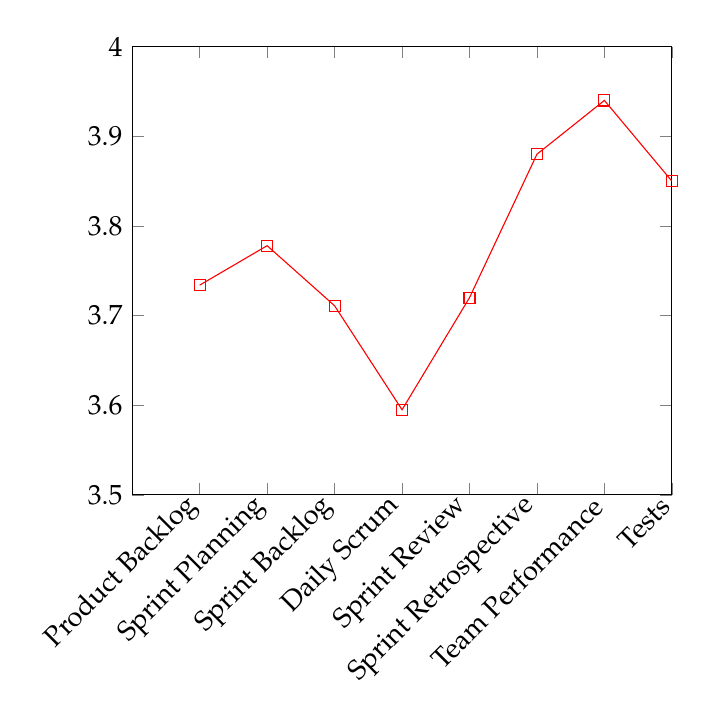
\begin{tikzpicture}
\begin{axis}[
    xmin=0, xmax=8,
    ymin=3.5, ymax=4,
    xtick=data,
    xticklabels={
        Product Backlog,
        Sprint Planning,
        Sprint Backlog,
        Daily Scrum,
        Sprint Review,
        Sprint Retrospective,
        Team Performance,
        Tests
    },
    x tick label style={rotate=45,anchor=east},
    legend pos=north west,
    grid style=dashed,
]
    
\addplot[
    color=red,
    mark=square,
]
coordinates {
    (1,3.734)
    (2,3.778)
    (3,3.711)
    (4,3.595)
    (5,3.72)
    (6,3.88)
    (7,3.94)
    (8,3.85)
};

\end{axis}
\end{tikzpicture}    
\decoRule
\caption[SCRUM metrics]{Scrum metric importance by activities, Source: \cite{PercPerfOfMetrForAgileScrumEnv}}
\label{fig:ScrumMetricsImportance}
\end{figure}

\noindent The figure (\ref{fig:ScrumMetricsImportance}) shows the mean of perceived importance 
of metrics that belong to a certain activity or category. 
From this one can conclude that me most important metrics are linked to 
team performance and the sprint retrospective.

\noindent The table \ref{tab:ScrumMetricsImportanceTable} illustrates the KPIs and their 
perceived importance within those categories. 
The mode represents the most frequent response given by the 
participants and the mean represents the mean value of all responses. In it's original form 
this table is quite large and was reduced to the KPIs relevant to this thesis. KPIs that were removed
were not relevant because they indicate performance in different SCRUM stages than planning and retrospective.
The aim of this thesis is to bring forth a method of evaluating SCRUM sprints automatically and only the KPIs listed 
in table \ref{tab:ScrumMetricsImportanceTable} were relevant for this stage of the process.


\begin{table}[]
    \centering
    \begin{tabular}{l l c c}
        \hline
        \textbf{Activity} & \textbf{Metric} & \textbf{Median} & \textbf{Mode} \\
        \hline
        Sprint backlog & Number of user stories & 4 & 5 \\
        & Number of tasks & 4 & 4 \\
        Sprint retrospective & Number of tasks in a sprint & 3 & 3 \\
        & Number of tasks completed in a sprint & 4 & 5 \\
        & Number of user stories completed in a sprint & 4 & 5 \\
        Team performance & Accuracy of estimation & 4 & 5 \\
        & Focus factor & 4 & 4 \\
        & Targeted value increase & 4 & 4 \\
        & Team member turnover & 4 & 3 \\
        & Team satisfaction & 4 & 4 \\
        & Velocity & 4 & 5 \\
        & Work capacity & 4 & 4 \\
    \end{tabular}
    \decoRule
    \caption[SCRUM metrics]{SCRUM metric importance by activities relevant to this thesis, Source: \cite{PercPerfOfMetrForAgileScrumEnv}}
    \label{tab:ScrumMetricsImportanceTable}
\end{table}

Based on the data, several conclusions can be made as a base for this thesis.
Both the number of completed tasks and the work done in story
points are crucial for a comprehensive sprint evaluation. 
Most metrics are objective and can be assessed without human intervention, 
with the exception of metrics like team satisfaction. 
The data also suggests that certain metrics, such as the number of 
planned user stories and tasks, 
should be determined before the sprint begins.

\subsubsection{Master thesis: Agile project health indicators}

In a master thesis published in 2019, Alexandra Esguerra states that 
performance indicators are essential for development and can be viewed as health checks for a project.
She lays out the challenges when selecting KPIs for a project and emphasizes that
the set of needed KPIs heavily depends on the team and the project itself.

A few different KPIs are mentioned and described as \textit{basis practices} in the analysis of agile methods in the following way:

\begin{itemize}
    \item \textbf{Velocity (Productivity)}: [...] You estimate this by defining the amount of completed user stories in very iteration. This measurement could help to estimate and see the overall productivity of the different teams.
    \item \textbf{Burn-down Chart}: This is a good tool to plan and monitor the progress in agile methods. It is also a way to show the remaining work. This [...] could be a guiding process to decision making on what to add or drop in case there is any delay on the project.
    \item \textbf{Schedule performance Indicator (SPI)}: This KPI will help to provide a clear view of the Schedule variance in the agile projects.
    \item \textbf{Cost performance indicator (CPI)}: This KPI will show how efficiently the project is spending the budget compared to how effectively it is planned to be spend.
\end{itemize}

The goal of the master thesis is to discover how KPIs can be applied in agile projects.
It also encourages readers to change traditional ways of thinking when it comes to project management
and shift to an agile mindset.

Some parts of this master thesis are also relevant to this bachelor thesis.
It can be learned that KPIs are essential in an agile context and that they depend 
heavily both on the project and the team that is using them.

\subsection*{Non - academic articles}

This section includes some mentions of articles on the internet written by bloggers and companies.
While the intention behind these articles may be of educational nature it is important that the reader
is informed that they are not of academical origin and are to be taken with a grain of salt.

Nevertheless they are relevant to this thesis to further push the point that teams require a spectrum of different 
SCRUM KPIs that are tailored to their specific needs.

\subsubsection*{SCRUM Metrics 101 - Atlassan}

The article 'SCRUM Metrics 101' which was published by Erika Sa on the website 
\textit{atlassian.com} describes how SCRUM metrics can enhance the 
effectiveness of the process \parencite{Atlassian2023}. 
The article argues that these metrics are essential for making informed 
decisions during and after a sprint. 
The article also stresses that there is no universal set of 
metrics that can work for any team using SCRUM. 
Each team needs to choose metrics that are useful to their situation. 

Erika Sa also explains that SCRUM metrics can be a great indicator of 
erformance but should not be the sole ingredient to analyze a team's performance. 
Harder to comprehend numbers like customer satisfaction should also be considered to
get the full picture.

In summary, the article advocates for a balanced,
data-driven approach to SCRUM metrics. 
It discourages teams from relying on intuition or gut 
feeling to improve their performance. 
Instead, it promotes the use of specific metrics to 
bring various dimensions of a team's 
effectiveness to the surface. The mentioned metrics for 
this are velocity, capacity, and quality of output.

\subsubsection*{11 Scrum Metrics and Their Value to Scrum Teams}
This article describes SCRUM metrics and how they are evaluated, 
focusing only on the categories Sprint planning, Daily SCRUM, 
and Sprint Retrospective \parencite{Sealights2023}. 
It describes the goals of KPIs used in SCRUM to measure the value of products 
delivered by the team and the effectiveness of the method. According to this website, 
KPIs may also help catch problems like dissatisfied developers early.
The article selects 11 KPIs and describes how they are helpful in combination with using SCRUM. 
Four of those are relevant to this thesis as they capture values relevant to SCRUM sprints.

\begin{itemize}
    \item \textbf{Sprint Goal success}:
    This KPI indicates whether the planned sprint goal has been met or not. It's simple to evaluate and quickly points out how well the team did.

    \item \textbf{Escaped defects and defect density}:
    Escaped defects describe every bug or issue that is encountered by a user in production. Defect density is a metric that shows the number of defects relative to the software size. Software size is typically the number of lines in the code.

    \item \textbf{Team Velocity}:
    The number of tickets completed by a team during a sprint is an indicator of how much work got done. If this number is averaged over previous sprints the KPI Velocity is computed. A rise in Velocity may indicate an increase in productivity.

    \item \textbf{Sprint Burndown}:
    The sprint burndown chart shows if the team is on schedule to complete the sprint or not. It shows the ideal trend line of the completed work for each day in comparison to the actual completed work.

\end{itemize}

Other metrics mentioned in the article are Time to Market, ROI, and Customer Satisfaction. Most of those are irrelevant for this thesis as they are not evaluated on each Sprint and therefore have no impact on improving performance sprint to sprint. Others like Team Satisfaction and Team Member Turnover do not apply as well because they are not objective numbers that can be computed and used as a solid base for performance evaluation.


\chapter{Research Methodology}

The following sections will describe how this project uses 
Design Science Research to ensure that the work is both practically 
relevant and academically sound.

\label{Chapter3}
\section{Overview of Design Science Research}

\enquote{
Simply stated, Design Science Research seeks to enhance
technology and science knowledge bases via the creation of innovative artifacts that solve
problems and improve the environment in which they are instantiated. The results of DSR include
both the newly designed artifacts and design knowledge (DK) that provide a fuller understanding
via design theories of why the artifacts enhance (or, disrupt) the relevant application contexts.
}  

  
- \cite{DesignScienceHevner}

\subsection{Characteristics of DSR}

DSR is a well-defined framework characterized by the following points and principles:

\begin{enumerate}
    \item \textbf{Artifact-Centric}: The core of DSR is the creation of artifacts. These can range from practical software applications and hardware systems to theoretical models and methods.
    \item \textbf{Problem-Solving}: DSR is inherently problem-oriented. It aims to address real-world challenges by developing practical solutions.
    \item \textbf{Iterative Development}: The methodology often involves an iterative process of design, development, and refinement. This allows for the continuous improvement of the artifact.
    \item \textbf{Evaluation}: A crucial aspect of DSR is the evaluation of the artifact to ensure it meets its intended objectives and solves the problem at hand.
    \item \textbf{Knowledge Contribution}: While the primary goal is problem-solving, DSR also aims to contribute to the body of knowledge by documenting the design process, the artifact, and the evaluation results.
\end{enumerate}

\subsection{Relevance to Research}

DSR is particularly relevant in fields like Information Systems, 
Computer Science, and Engineering, 
where the focus is not just on understanding problems 
but also on creating solutions. 
It provides a structured framework for the development 
and evaluation of artifacts, ensuring both practical 
utility and academic rigor.

\subsection{Methodological Steps}

Typically, a DSR project involves the following steps:

\begin{enumerate}
    \item \textbf{Problem Identification}: Understand and define the problem that needs solving.
    \item \textbf{Objective Setting}: Establish what the artifact aims to achieve.
    \item \textbf{Design \& Development}: Create the artifact based on the objectives.
    \item \textbf{Demonstration}: Show that the artifact works in a real-world scenario.
    \item \textbf{Evaluation}: Assess the artifact's effectiveness and efficiency.
    \item \textbf{Communication}: Document the results.
\end{enumerate}

The following sections will discuss how DSR will be used for this project and thesis
specifically.

\section{Artifact design and construction}
Artifact design in DSR heavily depends on the identification of the problem.
In the case of this thesis, the problem is described in Chapter \ref{Chapter1}.
After identifying the problem an objective was defined in 
section \ref{Chapter1-Objectives}. 
Based on this the application will be developed and evaluated. 
This thesis includes diagrams and possible scenarios the application should be able to handle in Chapter \ref{Chapter5}. 
These were created before the actual implementation as a guide
and then updated during the first development cycle. 
The construction of the artifact started with setting up a new software project and implementing the planned data models,
services, and APIs according to the specification created in the planning stage. 

\section{Artifact evaluation}

The most important factors for evaluating this artifact 
are the time a developer has to spend on creating a sprint
analysis and the completeness of the KPI spectrum. These factors are
determined by the partnering company to match the current method of evaluating
team performance.
Additionally, a 'good' artifact will also be defined by its usability, 
the easy process of deployment, and the lack of unexpected behavior. 
The definition of functional requirements and non-functional requirements will 
be helpful in determining these factors. 
More on evaluation in Chapter \ref{Chapter6}.
 
\chapter{Exploration of Performance Indicators} 

\label{Chapter4} 

\section{Methods of exploring the relevance of KPIs}

\subsection{Survey}

\subsubsection{Distribution}

A comprehensive survey was designed to gain insights 
into the perception and practical application of various KPIs in 
enhancing team performance. 
The survey was distributed among professionals within the partnering 
company and extended to colleagues working in other corporate 
environments to ensure a varied set of responses.
The survey was distributed electronically, ensuring 
ease of access for all participants. 

\subsubsection{Questions}

Two sections in the survey help find out more about the respondent and their views on KPIs. 
The following questions are presented to the participant:

\begin{itemize}
    \item Section 1: SCRUM experience
    \begin{itemize}
        \item Question 1: \textit{Do you have experience with SCRUM?}
        
        This question's purpose is to determine whether the respondent has had any experience with the SCRUM framework. This is to make sure that the following questions are only answered by experienced people.
        \item Question 2: \textit{How many years of experience do you have with SCRUM?}
        
        For those who have experience with SCRUM, this question aims to quantify the duration of their involvement. It helps in understanding how different levels of experience change the subsequent answers.
        \item Question 3: \textit{Which SCRUM roles have you primarily taken on?}
        
        This question is designed to identify the specific roles that participants have assumed within SCRUM teams.
    \end{itemize}

    \item Section 2: Evaluation of KPIs in the SCRUM context
    \begin{itemize}
        \item Question 4: \textit{How helpful do you find the following KPIs for SCRUM purposes?}
        
        Participants are presented with a list of KPIs and are asked to evaluate their helpfulness in the context of SCRUM. This question aims to gather data on the perceived relevance of each KPI.
        The list of KPIs includes the following items:

        \begin{itemize}
            \item Capacity: How many Story Points can a Team theoretically do in a Sprint?
            \item Number of planned tickets
            \item Number of done tickets
            \item Commitment: Story Points planned for a Sprint
            \item Overplanning ratio: Planned Story Points / Capacity
            \item Amount of done Story Points
            \item Velocity: Planned Story Points / Done Story Points
            \item Blocker Tickets: Number of 'emergency' tickets that got added during a Sprint
            \item Blocker Tickets done: Number of 'emergency' tickets that got done in the Sprint
            \item Additional Tickets: Tickets that got added unexpectedly during the Sprint
            \item Open Story Points: How many story points are not done at the end of a Sprint and what state are they in?
            \item Removed tickets: Tickets that got removed during a Sprint
        \end{itemize}

        \item Question 5: \textit{Is there a KPI not listed in our survey that you find helpful in the SCRUM context? If yes, please describe it.}

        This open-ended question allows respondents to identify and describe any additional KPIs not covered in the survey but deemed valuable in SCRUM.
    \end{itemize}
\end{itemize}

The results of the survey are presented later in section \ref{kpi-survey-results}.

\subsection{Criteria of evaluation} \label{CriteriaKPIEvaluation}

The evaluation of the helpfulness of a KPI is a multifaceted process.
In the context of this thesis, 
the criteria for evaluating the helpfulness of a KPI are the responses from the survey.
Below are the details of each criterion that may be considered when evaluating the helpfulness of a KPI:

\subsubsection{Quantifiable Impact}

A KPI is considered helpful if it yields quantifiable improvements 
in team performance, project delivery, or other relevant areas.

\subsubsection{Feasibility and accessibility}
The ease of measuring data for a KPI is essential. 
KPIs that require complex, time-consuming, or costly processes 
to measure may not be considered helpful.

\subsubsection{Clarity}

A helpful KPI is clear and easily understood 
by all team members. 
It should communicate information that aids in 
decision-making and performance improvement without ambiguity.

\subsubsection{Actionability}
The KPI should lead to actionable insights. 
It is considered helpful if the data collected and 
analyzed can be used to inform decisions and actions 
that enhance performance.

\subsubsection{Relevance over time}
The KPI's ability to remain relevant over an extended period is vital. 
It should adapt to a changing project and organization.

\subsection{Approach}\label{approach-kpi-explore}

Data from the survey is analyzed using analytical tools and techniques. 
Each KPI is scored based on its adherence to the criteria.

This comprehensive approach gives a feeling of what 
KPIs contribute tangible value to SCRUM practices and 
team performance and may be classified as more helpful. 
As has been argued in this thesis many times, 
there is no one-fits-all solution when it comes to analyzing SCRUM processes. 
That's why the purpose of this section is not to classify 
KPIs as helpful or not helpful but rather to get a feel for how this 
helpfulness can be subjectively evaluated to 
decide how to use the KPI in practice. 

\subsection{Expected outcome}
In anticipation of the survey results, 
a hypothesis is formulated to guide the analysis process. 
It is predicted that there will be a notable diversity in the 
KPIs preferred by different teams. 
This diversity is expected to highlight the participant's 
preference for clear and actional KPIs. Furthermore, 
it is hypothesized that most of the quantifiable KPIs 
favored by teams are not 'standard' or widely available. 
This means that they can not be read simply by looking at a 
SCRUM board but have to be computed separately.
This expected outcome will be refuted or validated as the 
detailed analysis of the survey data unfolds. 

\newpage

\section{Exploration of KPIs}

This section will lay out the data collected by the survey and discuss how it fits the expected outcome. 
It will also evaluate specific KPIs according to the criteria listed in section \ref{CriteriaKPIEvaluation}.
For this process KPIs will be selected from the survey data that had outliers in ratings to find reasons why that may be the case. 

\subsection{Survey data}\label{kpi-survey-results}

The survey was filled out by 64 participants of which 49 filled out the survey until the end and were relevant to this thesis. Irrelevant entries included people who did not have any experience with SCRUM. The data was exported and analyzed in different ways.

\subsubsection{Participants}

The participants were, for the most part, very experienced in SCRUM. 
26 stated that they used SCRUM for more than 4 years and 21 people chose an option placing them in the 1-4 years category, 
leaving only about 6\% for the category that has less than one year of experience in SCRUM. 
A pie graph in figure \ref{fig:scrum_experience_pie_chart} displays these results. 
SCRUM roles were distributed among the respondents in the following way: 
As expected about 68\% were SCRUM team members like developers and QA. 
The amount of SCRUM masters and product owners was about the same with 30.61\% product owners and 28.57\% 
SCRUM masters. 
Note that the participants could also select multiple SCRUM roles. 
That's why the total of all selected roles is 67 and not 49. 
The distribution of the roles is visualized in figure \ref{fig:scrum_roles_bar_chart}. 
Other options chosen for this question include \textit{Observer}, \textit{Product manager} \textit{Trainer}, and \textit{Observer of product development}.

\begin{figure}[!h]
    \centering
    \begin{tikzpicture}
        \pie[text=legend, color={mutedBlue, mutedGreen, mutedCoral, mutedPeach}]{
            6.12/less than 1 year (A1),
            14.29/1-2 years (A2),
            26.53/2-4 years (A3),
            53.06/4+ years (A4)
        }
    \end{tikzpicture}
    \caption{Answers to Question 2: How many years of experience do you have with SCRUM?}
    \label{fig:scrum_experience_pie_chart}
\end{figure}

\begin{figure}
    \centering
    \begin{tikzpicture}
        \begin{axis}[
            ybar,
            enlargelimits=0.15,
            legend style={at={(0.5,-0.2)}, anchor=north,legend columns=-1},
            ylabel={Count},
            symbolic x coords={Product Owner, SCRUM Team Member, SCRUM Master, Other},
            nodes near coords,
            nodes near coords align={vertical},
            x tick label style={rotate=45,anchor=east},
            every node near coord/.append style={text=black, font=\bfseries},
            ]
            \addplot+[fill=mutedBlue,draw=mutedBlue,text=mutedBlue] coordinates {(Product Owner,15)};
            \addplot+[fill=mutedGreen, draw=mutedGreen, text=mutedGreen] coordinates {(SCRUM Team Member,33)};
            \addplot+[fill=mutedCoral,draw=mutedCoral,text=mutedCoral] coordinates {(SCRUM Master,14)};
            \addplot+[fill=mutedPeach,draw=mutedPeach,text=mutedPeach] coordinates {(Other,5)};
        \end{axis}
    \end{tikzpicture}
    \caption{Answers to Question 3: Which SCRUM roles have you primarily taken on?}
    \label{fig:scrum_roles_bar_chart}
\end{figure}

\subsubsection{KPIs}

The biggest and most important part of the survey is the assessment 
of the perceived helpfulness of KPIs. 
The chosen ratings for each KPI follow a certain pattern that can be 
seen when calculating the average value. 
Some are perceived as more helpful like \textit{Capacity}, \textit{Planned Story Points} or \textit{Blocker Tickets}. 
Other KPIs like \textit{Planned Tickets} and \textit{Done Tickets} had mixed ratings and an average of about 2.8. 
Every rating was used on each KPI at least once which reinforces the idea that different teams and people require different KPIs. 
This can be seen by finding the maximum and minimum ratings for each KPI. 
These data points are documented in table \ref{tab:kpi_ratings}.

Some of the participants also decided to fill out the open-ended question at the end to bring in their own thoughts on what KPIs are helpful. Twelve of the respondents filled out this survey question. Since some answers were in German, they were translated into English to facilitate a universal understanding. The raw responses were then reduced to extract essential information, including the KPI name or a short description, the method of computation, and a detailed explanation where available. This process transformed the raw, verbose survey answers into concise, informative summaries of each proposed KPI. 

\begin{enumerate}
    \item \textbf{Quality of Refinements}
    \begin{itemize}
        \item \textit{Computation:} Compare the ratio of estimated to actual story points per ticket.
        \item \textit{Description:} Measures the accuracy of estimations made during refinements by comparing estimated story points to the actual story points required.
    \end{itemize}
    
    \item \textbf{Inter-Team Dependency Satisfaction}
    \begin{itemize}
        \item \textit{Computation:} Assess the KPI requirements of other teams and measure how well those are met.
        \item \textit{Description:} Evaluates how effectively a team meets the KPI requirements of other dependent teams.
    \end{itemize}

    \item \textbf{Pull Request and Release Count}
    \begin{itemize}
        \item \textit{Computation:} Count the number of pull requests for tickets in the sprint and the number of releases during/after the sprint.
        \item \textit{Description:} Monitors the development and deployment pace by counting pull requests and releases.
    \end{itemize}
    
    \item \textbf{Team Satisfaction and Bug to User Story Ratio}
    \begin{itemize}
        \item \textit{Computation:} Measure team satisfaction and compare the number of bugs to user stories in the backlog.
        \item \textit{Description:} Assesses team morale and the quality of work based on the prevalence of bugs.
    \end{itemize}

    \item \textbf{Story Stability}
    \begin{itemize}
        \item \textit{Computation:} Track changes made to the story during the sprint.
        \item \textit{Description:} Measures the frequency and extent of modifications to stories during development.
    \end{itemize}

    \item \textbf{QA Rejection Rate}
    \begin{itemize}
        \item \textit{Computation:} Calculate the frequency of issues sent back from QA.
        \item \textit{Description:} Assesses the quality of work based on how often QA rejects issues.
    \end{itemize}

    \item \textbf{Completion Rate}
    \begin{itemize}
        \item \textit{Computation:} Compare implemented story points to committed story points.
        \item \textit{Description:} Evaluates the team’s ability to complete committed work.
    \end{itemize}

    \item \textbf{Cycle Time, Lead Time, Predictability Measure}
    \begin{itemize}
        \item \textit{Computation:} Measure the time it takes to complete tasks and the percentage of stories accepted in the committed iteration.
        \item \textit{Description:} Evaluates efficiency and predictability in task completion and story acceptance.
    \end{itemize}

    \item \textbf{Technical Debt Ratio}
    \begin{itemize}
        \item \textit{Computation:} Measure the amount of technical debt or maintenance work included in each sprint.
        \item \textit{Description:} Ensures a balance between new feature development and maintenance work.
    \end{itemize}

    \item \textbf{Cycle Time and Throughput}
    \begin{itemize}
        \item \textit{Computation:} Avoid using tickets done per sprint; instead, measure cycle time and throughput.
        \item \textit{Description:} Provides a more accurate representation of velocity and productivity.
    \end{itemize}

    \item \textbf{User Stories to Technical Debt Ratio}
    \begin{itemize}
        \item \textit{Computation:} Compare the number of user stories implemented to the amount of technical debt addressed.
        \item \textit{Description:} Maintains a balance between feature development and technical debt resolution.
    \end{itemize}

    \item \textbf{Accepted Tickets Ratio}
    \begin{itemize}
        \item \textit{Computation:} Count tickets delivered and accepted by the Product Owner.
        \item \textit{Description:} Avoids a false sense of achievement by only counting tickets that are both delivered and accepted.
    \end{itemize}
\end{enumerate}


\begin{table}[!h]
    \centering
    \caption{KPI Ratings}
    \begin{tabular}{lcccc}
        \toprule
        KPI Abbreviation & Average Rating & Minimum Rating & Maximum Rating \\
        \midrule
        Capacity & 3.96 & 1.0 & 5.0 \\
        Done story points & 3.76 & 1.0 & 5.0 \\
        Commitment & 3.71 & 1.0 & 5.0 \\
        Velocity & 3.71 & 1.0 & 5.0 \\
        Open Story Points & 3.63 & 1.0 & 5.0 \\
        Blocker Tickets & 3.20 & 1.0 & 5.0 \\
        Overplanning ratio & 3.04 & 1.0 & 5.0 \\
        Additional Tickets & 2.90 & 1.0 & 5.0 \\
        Done Tickets & 2.85 & 1.0 & 5.0 \\
        Planned Tickets & 2.82 & 1.0 & 5.0 \\
        Blocker Done & 2.82 & 1.0 & 5.0 \\
        Removed Tickets & 2.45 & 1.0 & 5.0 \\
    \end{tabular}
    \decoRule
    \caption[SCRUM metric importance by activities]{SCRUM metric importance by activities}
    \label{tab:kpi_ratings}
\end{table}

\subsubsection{Correlations and outliers in the data}

There were no significant correlations in the survey data except ratings of KPIs that were similar. 
When computing the correlation matrix, 
two pairs of ratings for KPIs showed a high (>0.75) correlation. 
The statements that can be inferred by this fact is that the KPIs \textit{Number of planned Tickets} and \textit{Number of done Tickets} are often used together as well as \textit{Blocker Tickets} and \textit{Blocker Tickets done}. 
It makes sense to use these KPIs together so this correlation is not surprising.

Some KPIs discussed in the survey are going to be discussed further due to outliers in their ratings.

\paragraph{\textbf{Capacity}:} This KPI scored the highest on the survey. Reasons for that may be that it can directly influence how well a sprint planning goal is met. If the KPI is known at the sprint start, developers have an understanding of how much work they can complete during the sprint. It can be easily computed by averaging the amount of work done in past sprints. Ideally, it is measured in a universally applicable unit like story points. One drawback of this KPI is that it requires very much pre-existing data to be accurate. Averaging the amount of work done over a few sprints may lead to wrong conclusions. But over time, more and more measurements can be collected and this number should be more accurate.

\paragraph{\textbf{Done story points}:} A value representing the amount of work that got done in a sprint. The second most popular KPI \textit{Done story points} gives quick feedback to the development team and is easy to compute by counting the story points in every closed ticket. In combination with other KPIs, this can be an indicator of how well the sprint goal was reached or how much of the planned work is still not done. 

\paragraph{\textbf{Blocker Tickets \& Blocker Done}:} With a rating of about 3.20 and 2.82 these KPIs place sixth and second to last in the survey. The KPI \textit{Blocker Tickets} gives insight into how many emergency tickets were added after the planning. It is a metric of how unpredictable a sprint can be. If there are many blocker tickets in a sprint, this usually means planned work is left behind to prioritize the urgent blockers. It is very easy to compute since it is just a count of tickets that were marked as \textit{urgent} or \textit{blocker}. If this metric is often high, the development team might be able to plan less work before the sprint in order to leave some room for emergency tickets. The KPI \textit{Blocker Done} measures how many of those tickets were completed during the sprint. These two KPIs together can be important clues for planning a sprint. The greater the difference in values, the less leeway there was in the planning for emergency tickets. Among the opinions of the participants, these KPIs are not as helpful as others listed. 

\paragraph{\textbf{Removed Tickets}:} This KPI scored the lowest on the survey with a rating of 2.45. It computes a list of tickets that got removed during a sprint. This removal may be the result of a prioritized ticket being moved into the sprint retroactively for example. The KPI is hard to compute at the end of the sprint and requires a snapshot of the sprint before it was started. The value of this KPI may be relevant to some teams that have to explain to a customer why a ticket was not done in the sprint although it was planned, but otherwise, its applications seem to be limited.

\section{Practical implications}

What are the practical implications for SCRUM teams today considering the data gathered in this short research chapter? 
On the one hand, it seems as if the data collected supports the original hypotheses that quantifiable KPIs 
favored by teams are not 'basic' or 'commonly used' KPIs as labeled by literature discussed in section \ref{SOTAStudies}.
This is evident in two parts of the survey evaluation. 
Firstly, the fact that many suggestions for KPIs were made in response to question 5 and secondly that there were mixed ratings
for every KPI. This supports the original hypothesis and matches the expected outcome.
On the other hand, new insights were also gained. 
Most KPIs that are popular, as stated in studies discussed earlier in the literary review in section \ref{SOTAStudies}, 
are still favorites with most people. 
Unsurprisingly, which KPIs are seen as helpful depends on the years of experience and the SCRUM role. This is also supported by
a thesis discussed in section \ref{SOTAStudies} \parencite{AgileProjectHealthIndicatorsThesis}.

Overall, this exploration leads to the conclusion that different teams require different KPIs that cannot be modeled as static
if provided by a single application for multiple teams and different projects. 
Thus there seems to be a need for custom KPIs that cater to the specific requirements of a team.  
\chapter{Artifact design and features}
\label{Chapter5} 

In this chapter, the critical thought processes and decisions 
that shape the application architecture are documented. 
By exploring this chapter, readers will gain insights into the rationale behind the artifact structure and the reasons for selecting particular solutions over others.

\section{Capabilities and Requirements} 
\label{Requirements}

Requirements for the practical part of the thesis are defined before designing the artifact, following the DSR protocols. 
These are typically categorized into functional and non-functional requirements. 
Each plays a crucial role in the development process, 
contributing to the overall usability and performance of the application.

\subsection{Capabilities}

This section documents the process of finding specific requirements for the application.
This determines the starting point for model design later.
First, the main ideas are loosely written on paper and then reworked into 
requirements in cooperation with the organization introduced in section \ref{background-section}. 
The loose capabilities the application should have are as follows.

\textit{The artifact should be able to store templates for report creation. 
That means it should allow users to create templates or models to base their reports on. 
These templates should include information on how to get data and compute KPIs. 
To meet the requirement of creating custom KPIs, there has to be functionality available to create and manage custom KPIs.
The application should also provide the possibility to create graphical dashboards to 
present reports. 
Reports should also be comparable to other reports. 
Users should be able to manage who has access to their templates 
and what actions they can take in the context of their templates. 
The user creation and authentication are not handled by the application itself. 
Users are allowed to authenticate using OAUTH\footnote{\url{https://oauth.net/2/}}.
}

Further sections in this chapter will rework these statements into concrete requirements that can be used to evaluate the application.

\subsection{Functional Requirements}

Functional requirements are specific and describe the expected behavior of the artifact. 
They focus on what the system should do and include specifications of operations 
to take and outcomes to expect. 
This includes user interaction or interaction with other systems if needed. 

However, before defining functional requirements, actors have to be established. 
In the case of the envisioned application, the actors are the users of the application.
These users can be categorized into three different roles: Reader, Writer, and Admin. 
A higher-ranking role inherits the privileges of the roles below it. 
For instance, an Admin has all the rights of a Writer,
and a Writer possesses all the capabilities of a Reader.

For the artifact created in this thesis, the functional requirements are listed below: 

\compactSection{Log in}
\compactDescription{A Reader should be redirected to a login form on application startup. This form will allow the user to log in and guide them through the process. Once logged in, the user is redirected to the landing page.}
\compactSteps{
    \item Open the URL to the web application.
    \item Fill out the login form.
}
\compactOutcome{The Reader should be authenticated and redirected to the landing page.}

\compactSection{Get my models}
\compactDescription{A Reader should be able to retrieve all of their models and data. On a specific page of the application, all of the user's models are displayed in a table. There should be no model missing that the user has access to. There shouldn't be any models the user doesn't have access to.}
\compactSteps{
    \item Open the URL to the web application.
    \item Login.
    \item Go to the 'analysis' page.
    \item View the list of models.
}
\compactOutcome{The Reader should see all of their analysis models.}

\compactSection{Create a new model}
\compactDescription{The Reader should have the ability to create a new analysis model. If a new model is created, the user is automatically associated with the model as an administrative user.}
\compactSteps{
    \item Open the URL to the web application.
    \item Login.
    \item Go to the 'analysis' page.
    \item Click on 'Add a new model'.
    \item Select the new model.
    \item Click on 'Details'.
    \item Click on the tab 'Access'.
}
\compactOutcome{The Reader should now have a new model. The table under 'Access' only shows the user itself and that the Reader now has administrative privileges.}

\compactSection{View details of a model}
\compactDescription{Given a model, the Reader should be able to navigate to a detailed view of the model. This can be done by clicking a button.}
\compactSteps{
    \item Open the URL to the web application.
    \item Login.
    \item Go to the 'analysis' page.
    \item Select a model.
    \item Click on 'Details'.
}
\compactOutcome{The Reader should see a detailed page of their model.}

\compactSection{Change the KPI structure of a model}
\compactDescription{Given a model, an Editor should be able to create new KPIs, add new folders, and rename folders.}
\compactSteps{
    \item Open the URL to the web application.
    \item Login.
    \item Go to the 'analysis' page.
    \item Select a model.
    \item Click on 'Details'.
    \item Click on tab 'KPIs'.
    \item Click on 'Add new KPI'.
    \item Click on 'Add new folder'.
    \item Edit the name of a folder by clicking on the edit icon to the right of its name.
}
\compactOutcome{The Editor should be able to execute these steps without any errors.}

\compactSection{Delete a KPI or folder}
\compactDescription{Given a model, the Admin should be able to delete KPIs and folders. If a folder that contains KPIs is deleted, it should also delete the KPIs inside it.}
\compactSteps{
    \item Open the URL to the web application.
    \item Login.
    \item Go to the 'analysis' page.
    \item Select a model.
    \item Click on 'Details'.
    \item Click on tab 'KPIs'.
    \item Select a KPI.
    \item Delete the KPI.
    \item Delete a folder containing KPIs.
    \item KPI and the folder should be gone.
}
\compactOutcome{The Admin should be able to execute these steps without any errors.}

\compactSection{Edit KPI details}
\compactDescription{Given a model, the Editor should be able to edit the details of a given KPI.}
\compactSteps{
    \item Open the URL to the web application.
    \item Login.
    \item Go to the 'analysis' page.
    \item Select a model.
    \item Click on 'Details'.
    \item Click on tab 'KPIs'.
    \item Select an existing KPI or create a new KPI.
    \item Click on 'Details'.
    \item Edit the KPI name by clicking on the edit icon next to its name.
    \item Open the KPIs settings by switching to the 'Configuration' tab.
    \item Change the KPIs settings ('Basics' and 'Acceptable Items').
    \item Reload the web page.
}
\compactOutcome{The values after a page reload should be the values the Editor entered.}

\compactSection{Edit KPI expression}
\compactDescription{Given a model, the Editor should be able to edit the expression of a given KPI.}
\compactSteps{
    \item Open the URL to the web application.
    \item Login.
    \item Go to the 'analysis' page.
    \item Select a model.
    \item Click on 'Details'.
    \item Click on tab 'KPIs'.
    \item Select an existing KPI or create a new KPI.
    \item Click on 'Details'.
    \item Edit the KPIs expression by changing the type and changing the properties of the expression.
    \item Click on 'Save'.
    \item Reload the web page.
}
\compactOutcome{The values after a page reload should be the values the Editor entered.}

\compactSection{Add and edit a graphical dashboard}
\compactDescription{Given a model, the Editor should be able to add custom graphical dashboards to display report data.}
\compactSteps{
    \item Open the URL to the web application.
    \item Login.
    \item Go to the 'analysis' page.
    \item Select a model.
    \item Click on 'Details'.
    \item Click on the tab 'Settings'.
    \item Click on 'Add a new graphical layout'.
    \item A new layout should be visible in the list.
    \item Select the new layout.
    \item Click on 'Details'.
    \item Click on 'Change layout'.
    \item Add new widgets, resize, and reposition them.
}
\compactOutcome{The Editor should be able to execute these steps without any errors.}

\compactSection{Delete a graphical dashboard}
\compactDescription{Given a model, the Admin should be able to delete custom graphical dashboards.}
\compactSteps{
    \item Open the URL to the web application.
    \item Login.
    \item Go to the 'analysis' page.
    \item Select a model.
    \item Click on 'Details'.
    \item Click on the tab 'Settings'.
    \item Select a layout.
    \item Click on 'Delete'.
}
\compactOutcome{The deleted item should not show up in the list, even after a page reload.}

\compactSection{Create a report}
\compactDescription{Given a model, the Editor should be able to create a report.}
\compactSteps{
    \item Open the URL to the web application.
    \item Login.
    \item Go to the 'analysis' page.
    \item Select a model.
    \item Click on 'Details'.
    \item Switch to tab 'Reports'.
    \item Click on 'Create report'.
    \item Follow the steps to create a report.
}
\compactOutcome{The application should guide the Editor to create a report and the report should show up in the list once completed.}

\compactSection{View a report}
\compactDescription{Given a model, the Editor should be able to view a report in different ways.}
\compactSteps{
    \item Open the URL to the web application.
    \item Login.
    \item Go to the 'analysis' page.
    \item Select a model.
    \item Click on 'Details'.
    \item Switch to tab 'Reports'.
    \item Select a report.
    \item Click on 'Details'.
}
\compactOutcome{Multiple tabs feature different views of the report including a tabular view of all KPIs and a graphical view containing all configured dashboards.}

\compactSection{Delete a report}
\compactDescription{Given a model, the Admin should be able to delete a report.}
\compactSteps{
    \item Open the URL to the web application.
    \item Login.
    \item Go to the 'analysis' page.
    \item Select a model.
    \item Click on 'Details'.
    \item Switch to tab 'Reports'.
    \item Select a report.
    \item Click on 'Delete'.
}
\compactOutcome{The report is no longer listed on the model.}

\compactSection{Add a user to a model}
\compactDescription{Given a model, the Admin should be able to associate additional users to the model.}
\compactSteps{
    \item Open the URL to the web application.
    \item Login.
    \item Go to the 'analysis' page.
    \item Select a model.
    \item Click on 'Details'.
    \item Switch to the tab 'Access'.
    \item Click on 'Add user to model'.
    \item Enter the email address of the user you want to add.
}
\compactOutcome{Either the user is added to the list of associated users or a message is displayed that the user gets access to the model on the next login (If the user does not yet exist in the database he automatically gets access when they create their account).}

\compactSection{Change a user's permissions on a model}
\compactDescription{Given a model, the Admin should be able to change a user's permissions on the model.}
\compactSteps{
    \item Open the URL to the web application.
    \item Login.
    \item Go to the 'analysis' page.
    \item Select a model.
    \item Click on 'Details'.
    \item Switch to the tab 'Access'.
    \item Select a user.
    \item Click on the permission value.
    \item Select a new permission for the user.
}
\compactOutcome{The user's permissions have changed and they are only able to perform actions that are included in their permission.}

\compactSection{Remove a user from a model}
\compactDescription{Given a model, the Admin should be able to remove another user's access to the model.}
\compactSteps{
    \item Open the URL to the web application.
    \item Login.
    \item Go to the 'analysis' page.
    \item Select a model.
    \item Click on 'Details'.
    \item Switch to the tab 'Access'.
    \item Select a user.
    \item Click on 'Remove from model'.
}
\compactOutcome{The user is removed from the model and does not have access anymore.}

\subsection{Non functional Requirements}

Nonfunctional requirements are concerned with how the system performs under specific conditions. 
They do not directly capture specific functionalities but are essential in 
judging the usability, reliability, and performance of the system. 
For evaluating this later in chapter \ref{Chapter6}, a survey is crafted and distributed among the first users. 

Non-functional requirements to evaluate the application include:

\begin{itemize}
    \item Performance:
    \item \begin{itemize}
        \item The speed of the application should be adequate (no excessive loading or blocking)
        \item Users should not encounter a significant amount of lag
    \end{itemize}
    \item Usability:
    \item \begin{itemize}
        \item Users should be able to navigate through the application without any difficulties.
        \item Instructions inside the user interface should be clear and not misleading.
    \end{itemize}
    \item Reliability:
    \item \begin{itemize}
        \item The application should never freeze.
        \item Features and functions should work as described and expected.
    \end{itemize}
    \item Security:
    \item \begin{itemize}
        \item Users should not encounter any security or privacy issues.
    \end{itemize}
    \item Compatibility:
    \item \begin{itemize}
        \item Users should be able to access the application on their preferred web browser and operating system.
    \end{itemize}
    \item Overall experience:
    \item \begin{itemize}
        \item Users should be satisfied with the application overall.
    \end{itemize}
\end{itemize}

\section{Use cases}

Use cases of the application are defined in advance to help evaluate 
the produced artifact in the end. 
These use cases can be viewed as functional requirements that 
will be tested during the evaluation. 
The figures \ref{fig:use-cases-reader}, \ref{fig:use-cases-write} 
and \ref{fig:use-cases-admin} visualize each scenario for the three unique roles: Admin, Writer and Reader. 


All use cases are associated with requirements. 
They either have the same name as the requirement they represent or are annotated with the requirement that includes them in brackets behind their name.

\begin{figure}[!h]
    \centering
    \begin{tikzpicture}
      
        % Actor
        \umlactor[x=0, y=4]{Reader}
        
        % Use Cases Reader
        \umlusecase[x=6, y=7, name=getMyModels]{Get my Models}
        \umlusecase[x=6, y=6, name=getModelById]{View details of a model}
        \umlusecase[x=6, y=5, name=createModel]{Create a new Model}
        \umlusecase[x=6, y=4, name=getCustomQueries]{Get Custom Queries}
        \umlusecase[x=6, y=3, name=getRequiredQueries]{Get Required Queries}
        \umlusecase[x=6, y=2, name=getReport]{View a report}
        \umlusecase[x=6, y=1, name=logIn]{Log in}   
    
        
        % Associations
        \umlassoc{Reader}{getMyModels}
        \umlassoc{Reader}{getModelById}
        \umlassoc{Reader}{createModel}
        \umlassoc{Reader}{getCustomQueries}
        \umlassoc{Reader}{getRequiredQueries}
        \umlassoc{Reader}{logIn}
        \umlassoc{Reader}{getReport}
    \end{tikzpicture}
    \caption{Reader use cases of the application}
    \label{fig:use-cases-reader}
\end{figure}


\begin{figure}
    \centering
    \begin{tikzpicture}
      
        % Actor
        \umlactor[x=0, y=-3]{Writer}

        % Use Cases Writer
        \umlusecase[x=6, y=0, name=updateModel]{Update Model}
        \umlusecase[x=6, y=-1, name=createReport]{Create a report}
        \umlusecase[x=6, y=-2, name=createKPI]{Create KPI (Change the KPI structure of a model)}
        \umlusecase[x=6, y=-3, name=createLayout]{Create graphical layout (Add and edit a graphical dashboard)}
        \umlusecase[x=6, y=-4, name=updateKPI]{Update KPI (Edit KPI details)}
        \umlusecase[x=6, y=-5, name=addExpression]{Add Expression (Edit KPI Expression)}
        \umlusecase[x=6, y=-6, name=updateExpression]{Update Expression (Edit KPI Expression)}    
        \umlusecase[x=6, y=-7, name=updateLayout]{Update graphical layout (Add and edit a graphical dashboard)}
        
        % Associations
        \umlassoc{Writer}{updateModel}
        \umlassoc{Writer}{createReport}
        \umlassoc{Writer}{createKPI}
        \umlassoc{Writer}{createLayout}
        \umlassoc{Writer}{updateKPI}
        \umlassoc{Writer}{addExpression}
        \umlassoc{Writer}{updateExpression}
        \umlassoc{Writer}{updateLayout}
    \end{tikzpicture}
    \caption{Writer use cases of the application}
    \label{fig:use-cases-write}
\end{figure}

\begin{figure}
    \centering
    \begin{tikzpicture}
      
        % Actor
        \umlactor[x=0, y=-8]{Admin}

        % Use Cases Admin
        \umlusecase[x=6, y=-6, name=deleteKPI]{Delete KPI or folder}
        \umlusecase[x=6, y=-7, name=deleteReport]{Delete a report}
        \umlusecase[x=6, y=-8, name=deleteLayout]{Delete a graphical dashboard}
        \umlusecase[x=6, y=-9, name=addUser]{Add a user to a model}
        \umlusecase[x=6, y=-10, name=deleteUser]{Remove a user from a model}
        \umlusecase[x=6, y=-11, name=updateUser]{Change a user's permissions on a model}     
    
        
        % Associations
        \umlassoc{Admin}{deleteReport}
        \umlassoc{Admin}{deleteKPI}
        \umlassoc{Admin}{deleteLayout}
        \umlassoc{Admin}{addUser}
        \umlassoc{Admin}{deleteUser}
        \umlassoc{Admin}{updateUser}
    \end{tikzpicture}
    \caption{Admin use cases of the application}
    \label{fig:use-cases-admin}
\end{figure}


\newpage

\section{Model}

This section dives into the system's structure and its intended operations. 
First, the model is presented, detailing the primary components. 
Following that, various use cases illustrate the system in action, providing a comprehensive understanding of its functionality and interactions.

\subsection{Data model}

A central part of this application will be the data model behind it. 
Before actually implementing this model it is sketched out on paper. 
This step ensures that there is a clear picture of how the data elements relate and interact with each other. 
By mapping things out early, one can pinpoint potential issues and make necessary adjustments. 
Essentially, it's about laying a strong foundation from the get-go to ensure the app's long-term efficiency and adaptability. 
When the sketch is finished the model will be implemented code-first using an Object Relational Mapping (ORM) tool to map the coded model into a relational database. 
Most models will have a property called \code{Id} in which they store a Global Unique Identifier (GUID) value as the primary key for the relational database mapping. 
The diagrams presented in this section were designed with the Unified Modeling Language (UML) standard \footnote{UML standards document: \url{https://www.omg.org/spec/UML/2.5.1/PDF}} in mind. 
However, it is worth noting that while every effort is made to comply with the UML conventions there might be subtle differences in the representation. 

\begin{figure}
    \centering
    
        \begin{tikzpicture}
          
         \styledumlclass{AnalysisModel}{
          + Id : Guid \\
          + Name : string \\
          + ModelUsers : List<UserModel> \\
          + KPIs : List<KPI> \\
          + KPIFolders : List<KPIFolder> \\
          + Reports : List<Report> \\
          + Graphical : List<GraphicalConfiguration> \\
        }{}{0}{0}
        
        \styledumlclass{Expression}{
          + Id : Guid \\
          + Type : ExpressionType \\
          + ALLOWED\_QUERY\_TYPES : List<QueryReturnType> \\
          + QueryId : string \\
        }{
          + Evaluate(data : Dictionary<string, QueryResult>) : object? \\
          + GetRequiredQueries() : IEnumerable<string> \\
        }{0}{10}
        
        
        \styledumlclass{KPI}{
          + Id : Guid \\
          + Name : string \\
          + Unit : string \\
          + Expression : Expression \\
          + ShowInReport : bool \\
          + AcceptableValues : string? \\
          + AnalysisModelId : Guid? \\
          + FolderId : Guid? \\
        }{}{5}{5}
        
        \styledumlclass{KPIFolder}{
          + Id : Guid \\
          + Name : string \\
          + ParentFolderId : Guid \\
          + ModelId : Guid \\
          + KPIs : List<KPI> \\
          + SubFolders : List<KPIFolder> \\
        }{}{-5}{5}
        
        \styledumlclass{Report}{
          + Id : Guid \\
          + AnalysisModelId : Guid \\
          + Title : string \\
          + Notes : string \\
          + Created : long \\
        }{}{3}{-5}

        \styledumlclass{ReportData}{
        + Id: Guid \\
        + QueryResults: Dictionary<string, QueryResult> \\
        + KPIsAndValues: Dictionary<Guid, object?> \\
        }{}{4.25}{-10}

        \styledumlclass{GraphicalConfiguration}{
          + Id : Guid \\
          + Name : string \\
          + ModelId : Guid \\
          + Items : List<GraphicalReportItem> \\
        }{}{-4}{-5}
        
        \styledumlclass{GraphicalReportItem}{
          + Id : Guid \\
          + Type : GraphicalReportItemType \\
          + Name : string \\
          + Properties : GraphicalReportItemProperties \\
          + Layout : GraphicalReportItemLayout \\
          + DataSources : GraphicalItemDataSources \\
        }{}{-4}{-10}
        
        
        
        \umlassoc{KPI}{Expression}
        \umlaggreg{AnalysisModel}{KPI}
        \umlaggreg{AnalysisModel}{KPIFolder}
        \umlaggreg{AnalysisModel}{Report}
        \umlaggreg{AnalysisModel}{GraphicalConfiguration}
        \umlaggreg{KPIFolder}{KPI}
        \umlaggreg{KPIFolder}{KPIFolder}
        \umlaggreg{GraphicalConfiguration}{GraphicalReportItem}
        \umlassoc{Report}{ReportData}

        \end{tikzpicture}

    \caption{Relation KPIs and AnalysisModels}
    \label{fig:kpis-and-models}
\end{figure}


\subsubsection*{Analysis models}

The idea of this application is to have a way to design a schema or model that can be followed to evaluate performance indicators about a SCRUM sprint. 
The \code{AnalysisModel} data class is designed to do just that. 
It holds information about how to get and evaluate data. 
It also includes configuration on how to visualize data to present it to team members. 
A graphical representation shows the most important parts of the model in figure \ref{fig:kpis-and-models} after a brief description in the next paragraphs.

KPIs are an essential part of this thesis and have to be included in the data model. 
The classes \code{KPI} and \code{Expression} are designed to store details about KPIs and how to evaluate them. 
Also included in the \code{KPI} class is the configuration of the KPI like the unit to display and if it is supposed to show up on the final report. 
If a team has a lot of KPIs to calculate, storing them in a list can become very confusing. 
That's why the class \code{KPIFolder} is introduced so that a hierarchical structure can be offered. 
This allows KPIs to be organized more clearly.

\code{Expression}s are a way of telling the software how to evaluate raw data and reduce it to a KPI value. 
For this application, a few different types of expressions suffice. 
Further information on expressions is detailed in section \ref{model-expressions}.

To save actual reports and the data collected for them the \code{Report} class is designed. 
It relates to an \code{AnalysisModel} which in turn can relate to many instances of the \code{Report} class. 
The actual report data is held by the class \code{ReportData} which has a one-to-one relationship with the \code{Report} class as illustrated in figure \ref{fig:kpis-and-models}. 
Since the shape of the data saved in a report heavily depends on the model configuration the properties \code{QueryResults} and \code{KPIsAndValues}, 
which are holding the data, are saved in the database as JavaSscript Object Notation (JSON) binary data. 
This makes sure the data received when executing queries can be stored in its raw form, which in turn means that the evaluation of KPIs can be designed more flexibly. 

The class \code{GraphicalConfiguration} is used to store dashboards and layouts to display reports graphically. 
This way dashboards can be configured dynamically and presented to the team.

\subsubsection*{Expressions}\label{model-expressions}

\code{Expression}s are tightly coupled with \code{KPI}s and are used to evaluate sprint data and reduce it to values that can be displayed in a sprint report.
There are multiple types of expressions to evaluate different KPIs described in table \ref{tab:expression-types}.
These expressions can be in one of four different categories.
A \textit{Mathematical} expression is, unsurprisingly, used for mathematical operations.
It is used to combine other KPIs to calculate numeric values.
Aggregating an array of values can be achieved by using an expression of the \textit{Aggregation} category.
These expressions can reduce an array to a single value, calculating things like the maximum, minimum or average.
A \textit{Conditional} expression is used to filter a list of values and then perform an operation on them.
This allows for KPIs to count or sum values only if they meet certain conditions.
Lastly, \textit{Atomic} expressions can be used to represent simple, hard-set values or the plain value of a query. 
These expressions are modeled as a hierarchical structure with the \code{Expression} class as a base.
Their model is illustrated in figure \ref{fig:expression-hier}.

\begin{table}[!h]
    \centering
    \begin{tabular}{c c p{8cm}}
    \hline
    \textbf{Expression} & \textbf{Category} & \textbf{Description} \\
    \hline
    Add & Mathematical & Adds the result of two other KPIs together. \\
    \hline
    Div & Mathematical & Divides the result of two other KPIs. Useful for calculating ratios. \\
    \hline
    Multiply & Mathematical & Multiplies the result of two other KPIs. Useful to scale a value by a certain factor. \\
    \hline
    Subtract & Mathematical & Subtracts the result of two other KPIs. \\
    \hline
    Avg & Aggregation & Iterates over all list items extracting the given field. When all the values are extracted, the mathematical average is calculated. \\
    \hline
    Min & Aggregation & Iterates over all list items extracting the given field. When all the values are extracted, the mathematical minimum is calculated. \\
    \hline
    Max & Aggregation & Iterates over all work items extracting the given field. When all the values are extracted, the mathematical maximum is calculated. \\
    \hline
    Sum & Aggregation & Iterates over all work items extracting the given field. When all the values are extracted, the mathematical sum is calculated. \\
    \hline
    CountIfMultiple & Conditional & Count values in a list if they meet multiple conditions. \\
    \hline
    SumIfMultiple & Conditional & Sum values in a list if they meet multiple conditions. \\
    \hline
    CountIf & Conditional & Count values in a list if they meet a certain condition. \\
    \hline
    Plain & Atomic & Just return the plain result of a query. \\
    \hline
    Value & Atomic & Expression to define a simple numeric value. Useful for mathematical operations. \\
    \end{tabular}
    \caption{Descriptions of different expression types}
    \label{tab:expression-types}
\end{table}

\begin{figure}[!h]
    \centering
    \begin{tikzpicture}

        \styledumlclass{Expression}{
          + Id : Guid \\
          + Type : ExpressionType \\
          + QueryId: string \\
        }{
          + \textit{Evaluate(data : Dictionary<string, QueryResult>) : object?} \\
        }{0}{0}
        
        \styledumlclass{MathOperationExpression}{
            + Left: KPI \\
            + Right: KPI \\
        }{
            + \textit{DoOperation(double left, double right) : double} \\
        }{-5}{-8}
        
        \styledumlclass{AggregateExpression}{
          + Field : string \\
        }{
        }{5}{-8}
        
        \styledumlclass{DoIfMultipleExpression}{
          + Conditions : List<Condition> \\
          + Connection : ConditionConnection \\
          + ExtractField : string \\
        }{
            + \textit{Process(IEnumerable<object> conditionalItems): object?} \\
        }{0}{-12}
        
        \styledumlclass{PlainQueryExpression}{
        }{
        }{-5}{-4}

       \styledumlclass{NumericValueExpression}{
          + Value : double \\
        }{
        }{5}{-4}
        
        
        \umlinherit{MathOperationExpression}{Expression}
        \umlinherit{AggregateExpression}{Expression}
        \umlinherit{NumericValueExpression}{Expression}
        \umlinherit{DoIfMultipleExpression}{Expression}
        \umlinherit{PlainQueryExpression}{Expression}
        
        \end{tikzpicture}

    \caption{Expression types hierarchy}
    \label{fig:expression-hier}
\end{figure}

\subsubsection*{User management}

User management is crucial to an application that stores data multiple people should have access to. 
User access is controlled at the level of analysis models. 
This means a user can either have reading, writing or admin access to an \code{AnalysisModel} instance. 
Reading access privileges include read access to every related entity and the model itself.
Writing access works in the same manner and just adds writing access to all entities of the model. 
The only special access privileges are granted to administrative users. 
These allow a user to give other users access to the model and delete entities. 
Since a user can have access to multiple models and models should be able to be accessed by multiple users, an intermediate table is needed to model this relationship. 
This is illustrated in the diagram \ref{fig:user-model}.

\begin{figure}
    \centering
    \begin{tikzpicture}

        \styledumlclass{User}{
          + Id : Guid \\
          + DisplayName : string \\
          + EMail: string \\
        }{
        }{0}{3}
        
        \styledumlclass{RefreshToken}{
          + Token : string \\
          + IsActive : bool \\
        }{
        }{-5}{3}
        
        \styledumlclass{UserModel}{
          + Permission: ModelPermission \\
        }{
        }{0}{0}
        \styledumlclass{AnalysisModel}{
          + Id : Guid \\
          + Name : string \\
        }{}{-5}{0}

        \umlaggreg{AnalysisModel}{UserModel}
        \umlaggreg{User}{UserModel}
        \umlaggreg{User}{RefreshToken}
        
    \end{tikzpicture}
    
    \caption{User data model}
    \label{fig:user-model}
    
\end{figure}

\newpage

\section{Design considerations and choices}

\subsection{Implementation specifics}

There are multiple options for implementing an application to read and compile 
information from a digital SCRUM platform.
To meet the requirements of the partnering company this includes writing an extension for a 
specific platform and creating custom software that uses 
REST endpoints if the platform exposes any.

\subsubsection*{Extension for a SCRUM platform}
The requirement is to produce an artifact that will be used to extract 
data from the SCRUM platform Azure DevOps. 
Therefore a viable option would be to develop an extension for this platform.
Microsoft provides documentation on how to develop extensions for your 
organizational DevOps platform \footnote{Developing extensions for Azure: \url{https://learn.microsoft.com/en-us/azure/devops/extend/overview?view=azure-devops}}.
Simple authentication for users, storage provided by Azure and the 
accessibility of use speak in favor of this method.
The only downside, why it should be decided against, is that an extension for 
DevOps limits the functionality of the application to the Microsoft platform. 
If other things would also want to be integrated in the future, 
the application could not be extended in such a way that it 
also works with external applications. 
In addition, only developers could evaluate sprints and view the 
results because a Visual Studio license is required to access the platform.

\subsubsection*{Independent application}
An independent application can access work items and sprint info via a REST API provided by the most used SCRUM platforms like Atlassian Jira and Azure DevOps \parencite{TopTenScrum}.
If needed in the future, more platforms can be integrated into this 
application and it could be hosted anywhere. 
Another advantage is the free choice of the implementation language, 
which makes it much easier for a company to expand the application at a later date. 
A disadvantage is that the application has to be written from scratch. 
This means that communication with Azure services, user authentication, 
and data storage must both be designed and implemented. 
Nevertheless, it is a favorable choice.

\subsection{Application architecture}

An important decision is made to adopt a distributed application 
architecture. This is achieved by separating the front-end, back-end, and database into containerized parts. 
This choice is influenced by several factors and research pieces. 
One paper explores the performance of traditional VM deployments and 
contrasts them with the use of Linux containers. 
The authors used Kernel-based Virtual Machines (KVM) as a representative hypervisor and Docker as a container manager. 
The results show that containers result in equal or better 
performance than VMs in almost all cases \parencite{felter2015updated}. 
Another study compares the performance of Docker containers and VMs using 
different cloud vendors. 
Docker containers are found to be faster than KVMs and Xen VMs in terms of response time, 
download time, CPU processing time, and memory usage. 
The performance of Docker containers improves when scaled using the 
Kubernetes framework \parencite{chengeta2021comparing} which will also be 
the hosting choice for first evaluating the artifact. 
Relevant to this thesis and the decision made are the following points:

\begin{itemize}
    \item \textbf{Modern technology}: Distributed applications, especially when combined with containers, represent the cutting edge in software architecture. 
    \item \textbf{Scalable components}: One of the primary advantages of a distributed application is its scalability. Although it's not important for this thesis it's nice to have the option to scale as demand gets higher.
    \item \textbf{High availability}: Distributed architectures tend to offer better fault tolerance. Containerization further enhances this by allowing rapid redeployment of single components, ensuring minimal downtime.
    \item \textbf{Resource efficiency}: Containers are lightweight compared to traditional virtual machines. This means they start quickly and use fewer system resources. Multiple containers can be deployed onto a single machine which means that resources can be used more efficiently.
    \item \textbf{Consistent environments}: Containerization ensures that the application runs the same, regardless of where the container is deployed. This consistency can reduce the "it works on my machine" type of issues. 
    \item \textbf{Personal experience}: Familiarity with the technology stack is invaluable. Having prior experience with distributed systems and containers ensures a smoother development process.
\end{itemize}

Of course, the strategy of creating an application of containerized services is not suited for every application. 
This section illustrates that this is the best choice for this specific application and the partnering companies' hosting choices.

\subsection{Programming languages and frameworks}

This section will describe the kind of application that is envisioned.
It is established that it will be a web application, which leaves plenty of room for maneuver in terms of selecting the programming languages to implement it.
Selecting a programming language for a project is often influenced by the developer's previous experience. 
In many cases, developers lean towards languages they are already familiar with. 
This eliminates the need to learn a new language. 
This preference is not just a matter of comfort but also efficiency. 
Using a programming language known by the developer reduces errors, saves time,
and enhances the quality of the final artifact. 
Since the application is split into three parts two programming languages and frameworks have to be selected in addition to a database system.


\subsubsection*{Back-end}

The heart of the application is its API which is used to create and evaluate KPIs, 
issue and review Reports, and define dashboards for report presentation to a SCRUM team. 
ASP.NET is selected for this part of the application, 
which is a web application framework developed by Microsoft. 
ASP.NET is built on the Common Language Runtime (CLR), 
which means developers can write ASP.NET code using any supported .NET language like C\#, 
VB.NET, and F\#. The choice for this project is to use ASP.NET with C\# \footnote{ASP.NET documentation: \url{https://learn.microsoft.com/en-us/aspnet/core/?view=aspnetcore-7.0}}.

\subsubsection*{Database}

A relational database is used to store reports, 
KPIs, and other models that are needed for the application. 
The choice of provider is PostgreSQL because it's open source and easy to use with ASP.NET. 
The database schema is implemented code-first using an Object-Relational Mapping (ORM) framework for ASP.NET called Entity Framework. 
This framework automatically takes care of any migrations that may need to be issued to the schema and allows incremental creation of the model code first.

\subsubsection*{Front-end}

To present sprint metrics and data, configure how data is retrieved,
and manage user access a user interface is essential.
The front end of the application is coded in Typescript with the
extended capabilities of the library React by Facebook 
\footnote{React by Facebook: \url{https://react.dev}}. 
The user interface provides a method for the user to interact with the back-end API using controls rather than web requests which makes the application more accessible.  

\subsubsection*{Composition}

The final artifact consists of three docker images: 
one for the front end of the application, one for the back end,
and one for the database\footnote{Docker: \url{https://docs.docker.com/get-started/}}.
Locally, this can be run via a provided 'docker-compose' file but in production,
these images need to be hosted separately and configured in such a 
way that they know each other's location.

\section{Limitations}

The artifact is designed to have very few limitations when it comes to analyzing sprint data. 
The flexibility of having custom KPIs extends the types of metrics that can be extracted 
from Sprint by a lot. Some limitations however still exist:

\subsection*{Dependencies}

The produced artifact has dependencies that limit its use. The final application may only be used with SCRUM logging software that provides some sort of API to gather data. The data that is returned by this endpoint may only have a structured form (YAML, JSON). Examples of this are Azure DevOps Boards and Atlassian Jira.

\subsection*{Multiple organisations}
Pre-deployment of the artifact requires some configuration to be able to start. Each instance of the artifact has to know which endpoint to use to gather information about sprints. This makes the use of the artifact by multiple organizations impossible since they likely have different endpoints to query. Since the artifact is published as a lightweight Docker image it should be no problem to deploy one instance per organization. 

\section{Highlighted features}

This section provides a view into some highlighted features of the artifact. 
These are features that are characterized by the fact that they are more complex than others, 
are very relevant to understanding the artifact, 
and have special functionality. 

\subsection{Retrieving sprint data dynamically}

With the requirement to be able to request data from every possible SCRUM software that has some kind of API, 
some hurdles presented themselves for the design of the application. 

APIs from different providers have different specifications and also offer different possibilities. 
For example, Azure DevOps offers the option of installing a C\# package and reading out sprint data. 
Other providers such as Atlassan Jira offer a REST API. 
So it's important to find a way to support all methods.

To give the user the most flexibility but also restrict usage in some ways, 
an interface for sprint data retrieval is designed (Listing \ref{lst:devops-interface}).

\begin{lstlisting}[style=csharp, caption=Expression base class, label=lst:devops-interface]
public interface IDevOpsProviderService
{
    // Get all available queries provided by this SCRUM software 
    List<Query> GetQueries();
    // Get details of a single query  
    Query GetQueryById(string id);
    // Get parameters for the query that the query needs before executing  
    Task<List<QueryParameter>> GetQueryRuntimeParametersAsync(string queryId);
    // Execute a single query  
    Task<QueryResult> ExecuteQueryAsync(string queryId, Dictionary<string, object?> runtimeParameterValues);
    // Checks if the service has a valid configuration  
    bool HasValidConfiguration();
}
\end{lstlisting}

This allows the programmer to create standard classes for each major SCRUM provider starting with Azure DevOps. 
Additionally, if other, non-common software should be used to retrieve data the software can be extended by implementing this interface in a custom class and switching the used class out in the dependency injection configuration (Listing \ref{lst:devops-injection}). 

\begin{lstlisting}[style=csharp, caption=Expression base class, label=lst:devops-injection]
// Create ASP.Net application
var builder = WebApplication.CreateBuilder(args);

// Add configuration
var configFile = Path.Join(builder.Environment.ContentRootPath, "appsettings.json");
builder.Configuration.AddJsonFile(configFile, optional: false);

// Configure dependency injection service

// Add database configuration
builder.Services
    .AddDbContext<DataContext>(opts =>
    {

        var connectionString =  builder.Configuration
            .GetConnectionString("PostgresDatabase")

        opts.UseNpgsql(connectionString);
    });

// Add other services
// [...]
 
// Inject Azure DevOps provider service
builder.Services.AddScoped<IDevOpsProviderService, AzureDevOpsProviderService>();

\end{lstlisting}

This allows the workflow of creating a report to be the same regardless of the provider used. The user decides to create a sprint report and clicks the button in the UI, triggering that action. The user enters the name of the report and clicks 'Next'. After that, the UI requests an API endpoint called 'GetRequiredQueries' which yields all required queries by the model to create a report. 
After this list is returned, the front end requests an endpoint 'GetQueryRuntimeParameters' for each of the queries. Each of these requests returns a List of parameters for a query. These parameters are displayed for the user in a form. The user fills out the form and clicks 'Next'. The front-end sends a request to the back-end API endpoint 'CreateReport', including the query parameter values entered by the user. The back-end creates a report and saves it to the database. The report is then returned to the UI and the user can now see it. This behavior is also illustrated in figure \ref{fig:seq-queryparameters} in the form of a sequence diagram.

\begin{figure}
    \centering
    \begin{sequencediagram}
        \newinst{user}{User}
        \newinst[3]{ui}{UI}
        \newinst[3]{backend}{Backend}
        \newinst[3]{db}{Database}

        \mess{user}{Clicks create report button}{ui}
        \postlevel
        \mess{user}{Enters report name and clicks 'Next'}{ui}
        \mess{ui}{GetRequiredQueries}{backend}
        \mess{backend}{Queries list}{ui}
        
        \postlevel
        \begin{call}{ui}{For each query}{ui}{}
        \postlevel
            \mess{ui}{GetQueryParameters}{backend}
            \mess{backend}{Parameters list}{ui}
        \end{call}
        
        \mess{ui}{Displays parameters form}{user}
        \mess{user}{Fills out form and clicks 'Next'}{ui}
        \mess{ui}{CreateReport}{backend}
        \begin{call}{backend}{Save report}{db}{}
            \mess{db}{Report saved}{backend}
        \end{call}
        
        \mess{backend}{Returns report}{ui}
        \mess{ui}{Displays report}{user}
    \end{sequencediagram}
    \caption{Sequence diagram for creating a sprint report.}
    \label{fig:seq-queryparameters}
\end{figure}

\newpage

\subsection{Model associations of non-existent users}

\begin{figure}
    \centering
    \begin{tikzpicture}

         \styledumlclass{AnalysisModel}{
          + Id : Guid \\
          + Name : string \\
          + ModelUsers : List<UserModel> \\
          + KPIs : List<KPI> \\
          + KPIFolders : List<KPIFolder> \\
          + Reports : List<Report> \\
          + Graphical : List<GraphicalConfiguration> \\
        }{}{0}{0}

        \styledumlclass{ModelAssociationRequest}{
            + Id: Guid \\
            + Email: string \\
            + IssuedBy: User \\
            + IssuedAt: long \\
            + Completed: bool \\
            + CompletedAt: bool \\
            + Permission: ModelPermission \\
        }{}{0}{-5}

        \umlaggreg{AnalysisModel}{ModelAssociationRequest}
        
        \end{tikzpicture}

    \caption{ModelReportAssociation model}
    \label{fig:model-assoc}
\end{figure}


Since users are not stored in the application database and can use OAUTH to log in, a user may not exist by the time another user wants to add them to their model. This creates a need for the capability to associate a user automatically to a model when they first log in. This is realized by a class called \code{ModelAssociationRequest} (see figure \ref{fig:model-assoc}). This class is created when a user adds a non-existing user to their model. If a new user logs in all saved \code{ModelAssociationRequests} are searched for a matching email address. If one is found, the new user is automatically associated with the model listed in the \code{ModelAssociationRequest} entity. This behavior is illustrated in listing \ref{lst:user-update-method}.

\begin{lstlisting}[style=csharp, caption=Create user method, label=lst:user-update-method]
/// Method to create and update a user (user is created if id is not found)
public async Task<User> CreateOrUpdateUserAsync(User user)
{
    var existing = await m_context.Users.FindAsync(user.Id);
    // Check if user exists
    if (existing != null)
    {
        existing.DisplayName = user.DisplayName;
        existing.EMail = user.EMail.ToLowerInvariant();
    }
    else
    {
        user.EMail = user.EMail.ToLowerInvariant();
        existing = (await m_context.Users.AddAsync(user)).Entity;
        var modelAssocRequests = await m_context.ModelAssociationRequests
            .Where(x => x.Email == user.EMail && !x.Completed).ToListAsync();
        foreach (var request in modelAssocRequests)
        {
            var model = await m_context.AnalysisModels
                .FindAsync(request.ModelId);
            // Create association from user to model
            var userModel = new UserModel 
                { 
                    Model = model, 
                    User = existing, 
                    Permission = request.Permission, 
                };
            
            await m_context.UserModels.AddAsync(userModel);

            request.Completed = true;
            request.CompletedAt = DateTime.Now.ToUnixEpochTime();
        }
    }

    await m_context.SaveChangesAsync();
    return existing;
}
\end{lstlisting}


\subsection{Dynamic dashboard layouts}

\begin{figure}
    \centering
    \begin{tikzpicture}

         \styledumlclass{AnalysisModel}{
          + Id : Guid \\
          + Name : string \\
          + ModelUsers : List<UserModel> \\
          + KPIs : List<KPI> \\
          + KPIFolders : List<KPIFolder> \\
          + Reports : List<Report> \\
          + ModelAssociationRequests : List<ModelAssociationRequest> \\
        }{}{0}{0}

        \styledumlclass{GraphicalConfiguration}{
            + Id: Guid \\
            + Name: string \\
        }{}{-4}{-5}
        
        \styledumlclass{GraphicalConfigurationItem}{
            + Id: Guid \\
            + Type: GraphicalReportItemType \\
            + Name: string \\
            + Layout: GraphicalReportItemLayout \\
            + DataSources: GraphicalItemDataSources \\
        }{}{4}{-5}
        
        \styledumlclass{GraphicalReportItemLayout}{
            + Id: Guid \\
            + X: int \\
            + Y: int \\
            + W: int \\
            + H: int \\
            + MaxW: int \\
            + MaxH: int \\
            + MinW: int \\
            + MinH: int \\
        }{}{-4}{-10}
        
        \styledumlclass{GraphicalItemDataSources}{
            + Id: Guid \\
            + KPIs : List<Guid> \\
        }{}{4}{-10}

        \umlaggreg{AnalysisModel}{GraphicalConfiguration}
        \umlaggreg{GraphicalConfiguration}{GraphicalConfigurationItem}
        \umlassoc{GraphicalConfigurationItem}{GraphicalReportItemLayout}
        \umlassoc{GraphicalConfigurationItem}{GraphicalItemDataSources}
        
        \end{tikzpicture}

    \caption{Graphical layout model}
    \label{fig:graphical-items-layout}
\end{figure}


Custom configurable KPIs also require custom display options. 
Some KPIs may be better interpreted when viewed as a graph compared to just looking at the numeric value. 
The artifact should provide the possibility to create multiple dashboards for a model and these dashboards should have configurable layouts. 
The model constructed for this purpose is described as follows: 
An \code{AnalysisModel} can include many dashboards, which are represented by the entity class \code{GraphicalConfiguration}. 
Each \code{GraphicalConfiguration} may have multiple widgets modeled by the class \code{GraphicalReportItem}. 
These items include properties that can be used to save their size and position in the dashboard. 
The dashboards expand to the lower side of the screen and have a fixed number of twelve slots in the horizontal plane. 
Each widget on the dashboard can be scaled and re-positioned. 
This means developing the model to save layouts in the database and also finding a way to implement this in the front end of the application.
The model is illustrated in figure \ref{fig:graphical-items-layout} and some visualizations of the front-end code are included in figure \ref{fig:dashboards-config}. 
An applied version of the dashboard is illustrated in figure \ref{fig:appl-dashboard}. 
The different types of widgets also determine the maximum and minimum size of the widget. 
The data sources for the widget are mostly KPIs but for easier changes in the future, these properties have been abstracted to the class \code{GraphicalItemDataSources}.

\begin{figure}
    \centering
    \includegraphics[width=0.6\linewidth]{Figures/DashboardsConfig.png}
    \includegraphics[width=0.6\linewidth]{Figures/DashboardConfigWidgets.png}
    \caption{Dashobard widget types and configuration}
    \label{fig:dashboards-config}
\end{figure}

\begin{figure}
    \centering
    \includegraphics[width=1\linewidth]{Figures/DashboardApplication.png}
    \caption{Applied dashboard with real data}
    \label{fig:appl-dashboard}
\end{figure}

% Chapter Template

\chapter{Artifact Evaluation} 

\label{Chapter6} 

\section{Evaluation process and methods}

The final artifact will be evaluated by checking the requirements from section \ref{Requirements}. 
Functional requirements will be evaluated by a QA team member of a partnering organization (section \ref{background-section}).
The same organization will provide testers who fill out a survey to evaluate the nonfunctional requirements after using the artifact for two weeks. 
These results will be documented thoroughly in the next section.

\section{Evaluation results}

The evaluation of the functional requirements took place in two cycles, as the first evaluation was used to refine the artifact and remove any errors that were found. 
This section discusses both cycles and their results.

\subsection{Functional requirements}

The tested functionality includes every test case written for functional requirements. 
The test protocol produced is as follows:

\begin{itemize}
    \item \textbf{Login}: \textcolor{mutedGreen}{OK}
    \item \textbf{Get my models}: \textcolor{mutedGreen}{OK}
    \item \textbf{Create a new model}: \textcolor{mutedGreen}{OK}
    \item \textbf{View details of a model}: \textcolor{mutedGreen}{OK}
    \item \textbf{Change the KPI structure of a model}: \textcolor{mutedGreen}{OK}
    \item \textbf{Delete a KPI or folder}: \textcolor{mutedYellow}{Small error}
    \begin{itemize}
        \item Basic functionality OK
        \item If 'New KPI' is clicked immediately after a folder is deleted, an error is displayed on the screen.
    \end{itemize}
    \item \textbf{Edit KPI Details}: \textcolor{mutedGreen}{OK}
    \item \textbf{Edit KPI Expression}: \textcolor{mutedYellow}{Small error, display errors}
    \begin{itemize}
        \item Basic functionality OK
        \item Save button is broken after a reload of the expression form. 
        \item Small display errors: Misspelled texts in expression description, order of form fields does not match description, one form field is displayed but not used under the hood. 
    \end{itemize}
    \item \textbf{Add/Edit a graphical dashboard}: \textcolor{mutedPeach}{Not OK}
    \begin{itemize}
        \item Error displayed after adding a new dashboard. Reproduction: Click on a model, click on settings, add a new layout, add a new widget, and select a widget. Browser logs read \textit{TypeError: Cannot read properties of undefined (reading 'map')}
    \end{itemize}
    \item \textbf{Delete a graphical dashboard}: \textcolor{mutedYellow}{Small error}
    \begin{itemize}
        \item Works, but cannot confirm that it works on a dashboard with widgets because of the error in the test case \textit{Add/Edit a graphical dashboard}
    \end{itemize}
    \item \textbf{Create a report}: \textcolor{mutedGreen}{OK}
    \item \textbf{View a report}: \textcolor{mutedGreen}{OK}
    \begin{itemize}
        \item OK
        \item Comment: The description of the report is listed nowhere but can be entered when creating the report
    \end{itemize}
    \item \textbf{Delete a report}: \textcolor{mutedGreen}{OK}
    \item \textbf{Add a user to a model}: \textcolor{mutedGreen}{OK}
    \item \textbf{Change a user's permissions on a model}:\textcolor{mutedGreen}{OK}
    \begin{itemize}
        \item OK
        \item Comment: would be nice to show a message when permissions are changed.
    \end{itemize}
    \item \textbf{Remove a user from a model}: \textcolor{mutedPeach}{Not OK}
    \begin{itemize}
        \item Nothing happens when the \textit{Remove from model} button is clicked.
    \end{itemize}
\end{itemize}

The first test cycle revealed three small errors, two major errors and a few desired improvements.
The second cycle contained all test cases again to make sure functionality was not broken when implementing the changes for the previous errors:

\begin{itemize}
    \item \textbf{Login}: \textcolor{mutedGreen}{OK}
    \item \textbf{Get my models}: \textcolor{mutedGreen}{OK}
    \item \textbf{Create a new model}: \textcolor{mutedGreen}{OK}
    \item \textbf{View details of a model}: \textcolor{mutedGreen}{OK}
    \item \textbf{Change the KPI structure of a model}: \textcolor{mutedGreen}{OK}
    \item \textbf{Delete a KPI or folder}: \textcolor{mutedGreen}{OK}
    \item \textbf{Edit KPI Details}: \textcolor{mutedGreen}{OK}
    \item \textbf{Edit KPI Expression}: \textcolor{mutedGreen}{OK}
    \item \textbf{Add/Edit a graphical dashboard}: \textcolor{mutedGreen}{OK}
    \item \textbf{Delete a graphical dashboard}: \textcolor{mutedGreen}{OK}
    \item \textbf{Create a report}: \textcolor{mutedGreen}{OK}
    \item \textbf{View a report}: \textcolor{mutedGreen}{OK}
    \item \textbf{Delete a report}: \textcolor{mutedGreen}{OK}
    \item \textbf{Add a user to a model}: \textcolor{mutedGreen}{OK}
    \item \textbf{Change a user's permissions on a model}:\textcolor{mutedGreen}{OK}
    \item \textbf{Remove a user from a model}: \textcolor{mutedGreen}{OK}
\end{itemize}

The refinement of the artifact focused on eliminating the errors found in the first cycle. 
According to the second test report, the refinement was successful as no error could be reproduced when testing.

\subsection{Nonfunctional requirements}

As stated previously in section \ref{Requirements}, the nonfunctional requirements will be evaluated using a survey distributed among the first testers of the application. 
The following section dives deeper into the answers to the survey. 

Seven people who used the artifact extensively participated in this survey to rate this application and also gave some feedback for improvements.

\subsubsection{Ratings}

\begin{table}[!h]
    \centering
    \begin{tabular}{p{8cm} r}
    \hline
        \textbf{Question} & \textbf{Mean value} \\ 
     \hline
        \textbf{Performance} & \\
        How would you rate the speed of the application? & 4.83 \\
        Did you experience any lag or delays while using the application? & 4.67 \\
     \hline
        \textbf{Usability} & \\
        How easy was it to navigate through the application? & 4.17\\
        Were the instructions and labels within the application clear and understandable? & 3.83 \\
     \hline
        \textbf{Reliability} & \\
        How often did the application freeze? & 5.00 \\
     \hline
        \textbf{Compatibility} & \\
        How well did the application work on your device and operating system? & 5.00 \\
     \hline
        \textbf{Overall experience} & \\
        Overall, how satisfied are you with the application? & 4.17 \\
        
    \end{tabular}
    \caption{Survey questions for nonfunctional requirements}
    \label{tab:tool-ratings}
\end{table}

The mean of the ratings was calculated using the data analysis
tools discussed in section \ref{introduction-methods}.
The computed values are listed in table \ref{tab:tool-ratings}.
Some categorical data was also evaluated in this survey. 
While none of the participants found any security issues within the application, 
33\% noted that they encountered features that did not work the way they expected them to work.
The browsers that this application was tested on were Google Chrome\footnote{Google Chrome: \url{https://www.google.com/chrome/index.html}} with a majority of 83\% and Microsoft Edge\footnote{Microsoft Edge: \url{https://www.microsoft.com/en-us/edge?ep=194&form=MA13L3&es=40}} with 17\%. 

This data indicates that the application worked well overall and testers 
were especially satisfied in terms of compatibility and reliability. 
As predicted, without any experience in UX or UI there are some cases where participants were not able to intuitively figure out some features of the application. 
Some features were requested by the company after this first period of testing. 
While the application is functional and does everything that the organization needs, 
the requested features will be implemented outside of the context of this thesis. 

% Chapter Template

\chapter{Conclusion} 

\label{Chapter7} 

\section{Summary}

\section{Contribution}

It can be argued that this thesis contributes to the world of SCRUM and KPIs in two different ways: It extends the knowledge base about the demand for and usage of KPIs and contributes more practically to the actual evaluation and presentation of KPIs. These contributions will be further discussed in this section. 

\subsection{KPI usage and demand}

This thesis is yet another testimonial to how essential it is to use indicators to improve performance. Surveys, statistics, and the survey done in the context of this thesis all point to the fact that the people working with SCRUM find KPIs helpful for their process. These demands for KPIs differ vastly according to the team that answers these questions. It should be noted that some KPIs are likely to be more helpful and have a broader application for more teams. But it is also important to see that there is a demand by SCRUM actors for having custom KPIs to better analyze the performance of their specific team. All in all, this thesis helps define KPI usage and demands a little further.

\subsection{KPI evaluation}

The artifact produced during this thesis can ease the computation of complex KPIs by providing a user interface to do so. Teams can use this application to create templates for sprint reports. They can create custom KPIs and data sources to acquire data about their SCRUM process. To present the gathered data to their team members, custom dashboards can be created with ease. All these capabilities make it easier for teams to assess their performance and improve using custom metrics.


\section{Reflection on the process}   

%----------------------------------------------------------------------------------------
%	THESIS CONTENT - APPENDICES
%----------------------------------------------------------------------------------------

% \appendix % Cue to tell LaTeX that the following "chapters" are Appendices

% Include the appendices of the thesis as separate files from the Appendices folder
% Uncomment the lines as you write the Appendices

% \include{Appendices/AppendixA}
%\include{Appendices/AppendixB}
%\include{Appendices/AppendixC}

%----------------------------------------------------------------------------------------
%	BIBLIOGRAPHY
%----------------------------------------------------------------------------------------
\printbibliography

%----------------------------------------------------------------------------------------

\end{document}  
